\documentclass[11pt,a4paper]{article}
\usepackage[utf8]{inputenc}
\usepackage[T1]{fontenc}
\usepackage{amsmath,amssymb}
\usepackage{graphicx,booktabs,array,longtable}
\usepackage[margin=2.5cm]{geometry}
\usepackage{hyperref}
\usepackage{xurl}
\usepackage{setspace}
\emergencystretch=3em
\sloppy
\onehalfspacing
\setlength{\parskip}{0.4em}
\setlength{\parindent}{0pt}

\title{Matter-Dilution-Triggered Recollapse and Conditional Nonsingular Cycles in a Metastable Dark-Energy Model}
\author{Leon Sandler \\ Independent Researcher, Northbrook, Illinois, USA \\ sandler.leon@gmail.com   ·   ORCID 0009-0007-4584-808X}
\date{}
\begin{document}
\maketitle

\begin{abstract}
Can the dilution of matter end the cosmological expansion and start a new hot phase? We study a scalar field coupled to dark matter through $A(\varphi)=1+\varphi^2/2M^2$, which holds a vacuum with the observed dark-energy density while the dark-matter density exceeds a critical value and releases it into a negative vacuum once the expansion has diluted the matter. While the field is held, the homogeneous background reproduces $\Lambda$CDM to numerical accuracy ($w=-1$); after the release the expansion turns around tens of Gyr later. An intervention that freezes the density seen by the field keeps all 100 coupled models of a parameter grid expanding forever, whereas the uncoupled field with the same potential rolls before today for $\mu\ge300H_0$. With an effective loop-quantum-cosmology bounce, dissipation $\Upsilon\propto T^3$ and dark matter that obeys its own Boltzmann equation with a field-dependent mass, 100 consecutive cycles are integrated without resetting any variable. Each has a radiation-dominated bounce, freeze-out to the observed abundance, a matter era, a held dark-energy epoch of $5.28\pm0.01$ e-folds, a release and a turnaround, and the repeating cycle is an attracting fixed point of the bounce-to-bounce map. The cycle requires a bounce that rethermalizes the dark matter but stays below the percolation of the previous cycle's black holes, dissipation, inherited rather than regenerated shear and a coherent seed for the release; over stated parameter ranges these hold together in 6.8\% of draws. The cycle does not produce the observed primordial perturbations ($n_s\approx3$), so the results are conditional background solutions, not an observationally complete cosmology.
\end{abstract}
\noindent\textbf{Keywords:} \emph{cyclic cosmology; nonsingular bounce; dark energy; coupled dark matter; symmetron; recollapse; Boltzmann equation; dissipation; anisotropy}

\section{Introduction}
The idea examined here reverses a common intuition. The dilution of matter is usually the end state of cosmic evolution, the approach to heat death in an accelerating universe. Here it is the trigger. If the dark energy is the energy of a vacuum held in place by dark matter, the emptying of the universe destabilizes it, and the expansion can turn into contraction, a bounce and a new hot phase. The paper asks what such a cycle requires, computes it without prescribed steps, and identifies the conditions under which it fails.

Cyclic and bouncing cosmologies have a long history [1, 2, 3, 4, 5, 6, 7]. Most specify the mechanism that ends the expansion separately from the observed universe, and many reset some variable between cycles. Three ingredients used here are established. Scalar fields coupled to matter whose effective potential depends on the local density are known from chameleon and symmetron screening [8, 9, 10] and from coupled dark energy [11]. An effective bounce at high density follows from loop quantum cosmology [12, 13, 14]. Thermal dissipation of scalar energy [15] and thermal freeze-out [16, 17] are standard early-universe physics. What is examined here is their combination into a cycle that contains a hot big bang and an epoch like ours, followed without resets, with control experiments that remove each ingredient and an explicit map of the conditions under which the cycle fails.

Four results are reported. (i) A symmetron-type coupling to dark matter holds the observed dark energy while the matter density is above a critical value, with a $\Lambda$CDM past, and releases it by dilution into a negative vacuum, which ends the expansion; an exact energy relation fixes how much the dark-matter mass must grow at the release (Sections 2, 3). (ii) Intervention tests show that, within the model, dilution decides when the expansion ends; a negative vacuum without the coupling also recollapses but cannot reproduce the observed past over most of the parameter range, so the coupling is not claimed to be the only possible cause of a recollapse (Section 3.3). (iii) With an effective bounce, thermal dissipation and Boltzmann dark matter, 100 consecutive cycles are integrated without any reset; the repeating cycle is an attracting fixed point of a bounce-to-bounce map, and the length of its dark-energy epoch has a closed form (Section 5). (iv) The conditions are explicit: a bounce hot enough to rethermalize the dark matter and cold enough to keep black holes from percolating, dissipation, inherited rather than regenerated anisotropy, and a coherent seed for the release; their joint viability over stated parameter ranges is quantified (Sections 4, 6).

\subsection{Relation to previous work}
Tolman showed that a closed universe that bounces with entropy production grows from cycle to cycle [1], and the entropy problem has remained the central obstacle to cyclic models since: a cycle that returns to the same state must dispose of the entropy it produces, and geodesically complete cyclic cosmologies face constraints from it [18]. The ekpyrotic and cyclic models of Steinhardt and Turok end each expansion with a scalar that rolls to negative energy and handle the entropy by an exponential expansion that dilutes it [4, 19]; Penrose's conformal cyclic cosmology matches the remote future of one aeon to the big bang of the next [2]; pre-big-bang and bouncing scenarios replace the singularity by a bounce of various origins [3, 6, 7, 5]. Oscillating models with a bounce show a hysteresis in which successive cycles grow [20]. The present model shares the negative-vacuum turnaround with the cyclic models and Tolman's growth law, but differs in three respects. The turnaround is not imposed by a potential that the field rolls down at a prescribed time; it is triggered by the dilution of the dark matter that held the vacuum, so that the observed dark energy is the held vacuum itself. The entropy is not diluted away but absorbed in the growth of the next cycle while the local thermal history, set by freeze-out, repeats. And no variable is reset between cycles: the dark-matter abundance and the restoration of the vacuum are outputs of the equations.

Couplings of a scalar to matter that make its effective potential density dependent are the basis of chameleon [8] and symmetron [9, 10] screening and of coupled dark energy [11]; in the symmetron the symmetric point is held at high density and broken at low density, exactly the mechanism used here, but applied to local screening rather than to the cosmological vacuum energy. The effective bounce of loop quantum cosmology [12, 13, 14] provides a nonsingular continuation at a critical density; it is used here as a prescription. Thermal dissipation of scalar energy is the mechanism of warm inflation [15], and thermal freeze-out [16, 17] sets the dark-matter abundance. None of these ingredients is new; their combination into a cycle that contains an epoch like ours is.

The scope is stated at the outset. The bounce is an effective prescription, not a derivation; the dynamics are homogeneous; and the cycle does not produce the observed primordial perturbations (Section 7). The results are therefore conditional solutions for the background cosmology. A distinct possibility, in which dilution makes the held vacuum metastable and it decays by localized bubble nucleation, raises separate questions, including whether a smooth dark-matter density describes the field on the much shorter length scale of a vacuum wall; it is examined in a companion paper [21] and is not used here.

\section{The matter-coupled metastable vacuum}
\subsection{Action and effective potential}
The scalar is coupled conformally to dark matter only; baryons and radiation are uncoupled, which avoids the stringent visible-sector fifth-force tests:

\begin{equation}
S=\int d^4x\sqrt{-g}\left[\frac{M_{\rm Pl}^2R}{2}-\frac{1}{2}(\nabla\varphi)^2-V_0(\varphi)\right]+S_{\rm dm}\left[A^2(\varphi)g_{\mu\nu},\psi_{\rm dm}\right]
\end{equation}
For pressureless dark matter the conserved Einstein-frame density $\rho_*=\rho_{*,0}a^{-3}$ enters the field equation through the effective potential, and the physical dark-matter density is $A(\varphi)\rho_*$ [11, 9]. With

\begin{equation}\begin{gathered}
V_0(\varphi)=V_c-\frac{\mu^2}{2}\varphi^2+\frac{\lambda}{4}\varphi^4,\qquad A(\varphi)=1+\frac{\varphi^2}{2M^2},\\
V_{\rm eff}=V_0+\rho_*A(\varphi)
\end{gathered}\end{equation}
the effective mass at the symmetric point is $m_{\rm eff}^2=\rho_*/M^2-\mu^2$. The point $\varphi=0$, with vacuum energy $V_c>0$, is held while $\rho_*>\rho_{\rm crit}=\mu^2M^2$ and released when the expansion dilutes the matter below it, at

\begin{equation}
a_c=\left(\frac{\rho_{*,0}}{\mu^2M^2}\right)^{1/3},\qquad V_c-V_0(v)=\frac{\mu^2v^2}{4}=\frac{A(v)-1}{2}\,\rho_{\rm crit}
\end{equation}
This is the symmetron form [9, 10] with two changes: the coupling is to dark matter, and the broken vacua $\varphi=\pm v$, $v^2=\mu^2/\lambda$, carry negative energy $V_0(v)=-qV_c$. Today $V_c=3\Omega_\Lambda H_0^2M_{\rm Pl}^2$, so the model reproduces the observed dark energy while it is held, and $a_c>1$ is required for it to be held now. The second relation is exact and has a consequence that cannot be avoided: the vacuum energy given up at the release equals half the coupling energy stored at the critical density, and since $\rho_{\rm crit}<\rho_{\rm dm,0}<V_c$, a release into a negative vacuum needs $A(v)-1>2V_c/\rho_{\rm crit}$, i.e., the dark-matter mass must grow severalfold once the field rolls ($A(v)=85$ for $a_c=2$, $q=1$; $6.1$--$7.2\times10^{3}$ over the parameter grid below). At $\varphi=0$ the coupling $\beta=M_{\rm Pl}\,d\ln A/d\varphi$ vanishes, so the homogeneous background carries no fifth force today. The background equations (flat, general relativity) are

\begin{equation}
3M_{\rm Pl}^2H^2=\rho_r+\rho_b+A\rho_*+\frac{\dot\varphi^2}{2}+V_0,\qquad \ddot\varphi+3H\dot\varphi+V_0'+\rho_*A'=0,\qquad \dot\rho_*=-3H\rho_*
\end{equation}
with $\dot H=-(\tfrac43\rho_r+\rho_b+A\rho_*+\dot\varphi^2)/2M_{\rm Pl}^2$. Total stress-energy is conserved: the scalar and the coupled matter exchange energy through $A'$, and the coupling energy is counted once, in $A\rho_*$. The equations are integrated from recombination ($z=1100$) with the field at the de Sitter quantum floor, $\varphi_0=10^{-60}v$ (approximately $H/2\pi$ in Planck units), in units of $H_0$ and $M_{\rm Pl}$ (dilution\_background.py).

The comparison with $\Lambda$CDM has a definite scope, and three levels are distinguished. (i) The homogeneous background: while the field is held, the background reproduces $\Lambda$CDM to numerical accuracy (Section 3.1). (ii) Linear perturbations: around $\bar\varphi=0$ the field fluctuation has the mass $m_{\rm eff}$ and is not sourced by dark-matter density perturbations at first order, because the source term $\rho_*A'(\bar\varphi)\delta$ vanishes; the dark matter therefore feels no linear fifth force. This has not been followed through structure formation, where second-order terms and the time dependence of $m_{\rm eff}$ enter. (iii) Low-density regions: where the local density stays below $\rho_{\rm crit}$ over more than a Compton length, as in the deepest voids, the held point is locally unstable and the field can roll there before it does in the mean (Section 7.1). The statement established here is therefore: the homogeneous background reproduces $\Lambda$CDM to numerical accuracy while the scalar remains at the symmetric point; perturbative and environmental deviations remain to be tested. The smooth density used as the source is accurate in this model, because the field's Compton length is cosmological (17 Mpc today for $a_c=2$, $\mu=100H_0$, and of order a kiloparsec at recombination), so it averages over an enormous number of dark-matter particles.

\subsection{Coherence of the release}
The release is a classical (spinodal) roll: the held point loses stability at $\rho_{\rm crit}$ exactly when the broken minima appear, and the occupied minimum is never metastable (vacuum\_phase\_map.py). The sign of the roll must therefore be set coherently over the region; otherwise domain walls between $+v$ and $-v$ form, and they would carry up to 21\% of the critical density per Hubble volume. In the cycles of Section 5 the field restored by the hot phase starts each held epoch 2 to 19 times above the Hubble-scale quantum fluctuation $H_\Lambda/2\pi$, a marginal margin; any explicit breaking of $\varphi\to-\varphi$ with a tilt $\epsilon\gtrsim4\times10^{-64}\,\mu^2v$ sets the sign coherently, and this is assumed. Matter inhomogeneity does not produce sharp interfaces: the field averages the density over its Compton length (148 Mpc at release), where linear fluctuations are $\sigma_R=0.062$, so the release time varies by $\delta a/a\approx0.021$ between such regions and the homogeneous treatment holds to that accuracy.

\section{Density-triggered transition and cosmological turnaround}
\subsection{Release and recollapse}
Three models are compared with identical initial data: $\Lambda$CDM (A), the uncoupled scalar with the same potential (B, the control) and the coupled scalar (C). For the reference case $a_c=2$, $\mu=100H_0$, $q=1$ (Fig. 1), $\Lambda$CDM expands forever. The coupled field stays at $|\varphi|/v=4.2\times10^{-64}$ up to the present, so the homogeneous past history is that of $\Lambda$CDM ($w_0=-1$ to all digits; $H(a)$ agrees with $\Lambda$CDM to the integration accuracy), is released after $a_c$, rolls at $a=8.25$ and turns the expansion around at $a=10.64$, 46 Gyr from now. The uncoupled control has been unstable since recombination and turns around at $a=2.05$, 17 Gyr from now.

Over a grid of 100 coupled models ($a_c=1.25$--$5$, $\mu=3$--$300H_0$, $q$ from $-0.5$ to $10$) every one reaches the present with the vacuum held; 75 release into a negative vacuum and recollapse, and the 25 with $q<0$ settle in a lower de Sitter vacuum and expand forever (Fig. 2b, Table 1). The control rolls before today for $\mu\ge300H_0$, so it cannot describe the observed universe there, while the coupled model can at every $\mu$. The coupling is what makes a late release compatible with an observed $\Lambda$CDM past. The release is not instantaneous: the field grows from the quantum floor at a rate of order $\mu$, so the roll lags $a_c$ by approximately $\ln(v/\varphi_0)/\mu$ Hubble times, from $a=2.69$ to $8.25$ for seeds $10^{-6}$ to $10^{-60}v$; the control rolls before today for every seed above $10^{-40}v$ (Fig. 2c).

The release changes the matter content as well as the vacuum. Once the field rolls to $v$ the dark-matter mass grows by $A(v)$, so the physical dark-matter density jumps by that factor while the vacuum energy falls from $V_c$ to $-qV_c$; the energy relation of Section 2.1 makes the two changes balance at the release. The universe then decelerates, and the turnaround occurs when the diluting matter and radiation no longer compensate the negative vacuum, $A(v)\rho_*+\rho_b+\rho_r\simeq qV_c$, within a fraction of a Hubble time of the release for $q=O(1)$; for $q<0$ the field settles in a lower de Sitter vacuum and the expansion continues. The model therefore makes the timing of the end of the expansion a property of the matter density, not of a clock in the potential: the release occurs when $\rho_*$ falls to $\rho_{\rm crit}$, whatever the history before it.

\begin{table}[htbp]\centering\small
\caption{Release and turnaround of the coupled model and the uncoupled control ($a_c=2$, $q=1$, seed $10^{-60}v$ at $z=1100$). Times from today; $A(v)$ is the factor by which the dark-matter mass grows after the release.}
\begin{tabular}{llllll}
\toprule
$\mu/H_0$ & roll, $a$ & turnaround, $a$ & turnaround (Gyr) & control turnaround, $a$ & $A(v)$ \\ \midrule
3 & 1.63e+26 & 1.88e+26 & 1061 & 4.28e+24 & 85 \\
10 & 1.76e+06 & 2.09e+06 & 259 & 2.84e+05 & 85 \\
30 & 156 & 195 & 96 & 34.9 & 85 \\
100 & 8.25 & 10.6 & 46 & 2.05 & 85 \\
300 & 3.57 & 4.7 & 32 & rolled before today & 85 \\
\bottomrule
\end{tabular}
\end{table}
\begin{figure}[htbp]\centering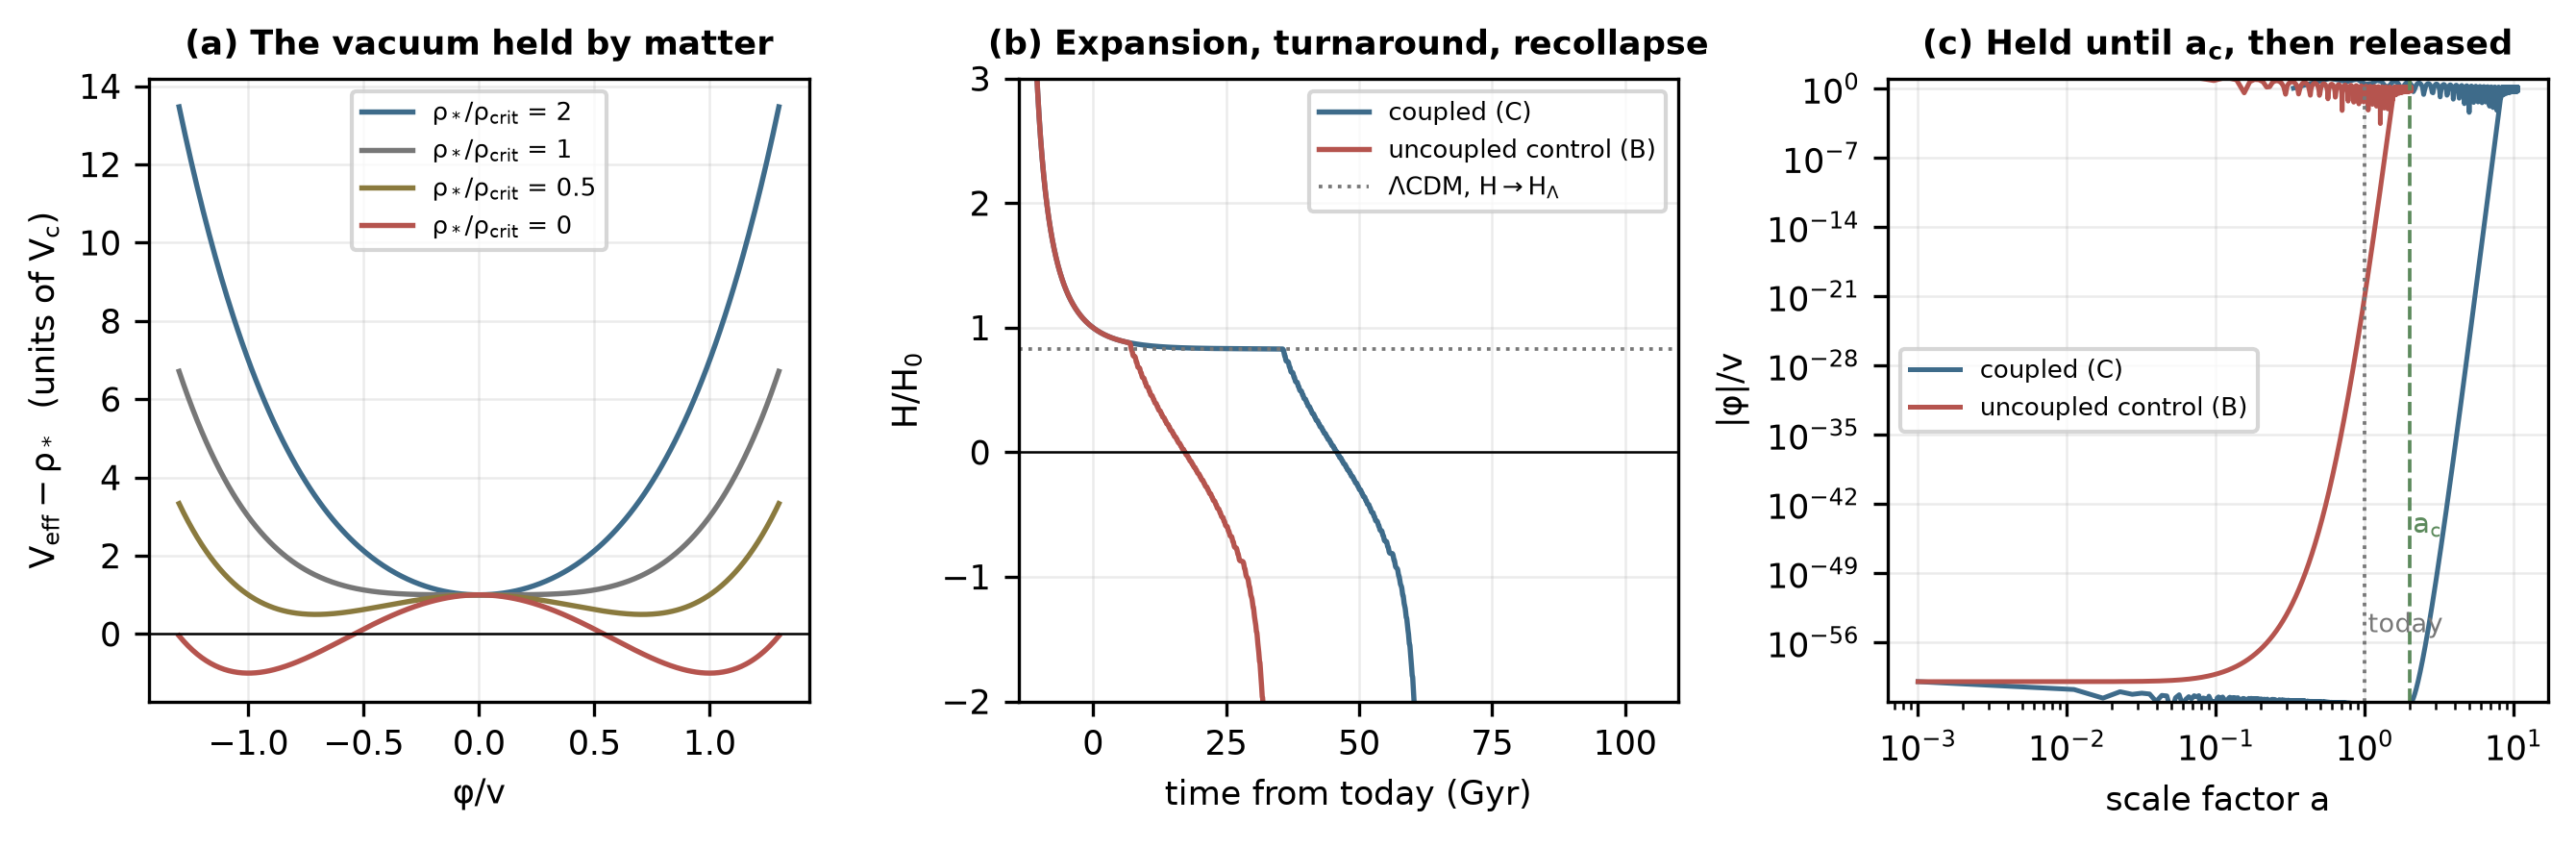
\includegraphics[width=1.00\textwidth]{../figures/fig13_matter_held_vacuum.png}\caption{The matter-held vacuum ($a_c=2$, $\mu=100H_0$, $q=1$). (a) Effective potential for several matter densities; the symmetric point, with energy $V_c$, is a minimum while $\rho_*>\rho_{\rm crit}$. (b) Hubble rate against time from today for the coupled model, the uncoupled control and $\Lambda$CDM. (c) Field amplitude from recombination: the coupled field is held at the quantum floor until $a_c$, the control grows from the start.}\end{figure}
\subsection{Cooling or dilution?}
A thermal mass $cT^2\varphi^2/2$ from a bath of temperature $T$ acts in the same way: the symmetric point is held while $\rho_*/\rho_{\rm crit}+(T/T_c)^2>1$, $T_c=\mu/\sqrt c$, and the possible triggers are compared in Fig. 2a. With the critical scale factor set to 2 for each, matter alone releases the field at $a=2$, temperature alone at $a=2$, both together at $a=2.65$, and all three recollapse ($a=10.6$, $11.9$ and $14.9$). Mathematically, then, cooling could trigger the release; physically it cannot. In physical units $\sqrt c=\mu a_T/T_0$, so a release at $a_T\sim2$ with $\mu=100H_0$ needs $\sqrt c=1.2\times10^{-27}$, and a scalar with so weak a coupling interacts with the bath at a rate $\sim c^2T\approx4\times10^{-79}\,H_0$: it never reaches equilibrium, and the thermal mass is never established. A coupling strong enough for equilibrium today, $\sqrt c>5\times10^{-8}$, holds the field until $a_T\sim8\times10^{19}$. The two requirements exclude each other by twenty orders of magnitude. Cooling does not trigger the release; dilution of dark matter can.

\begin{figure}[htbp]\centering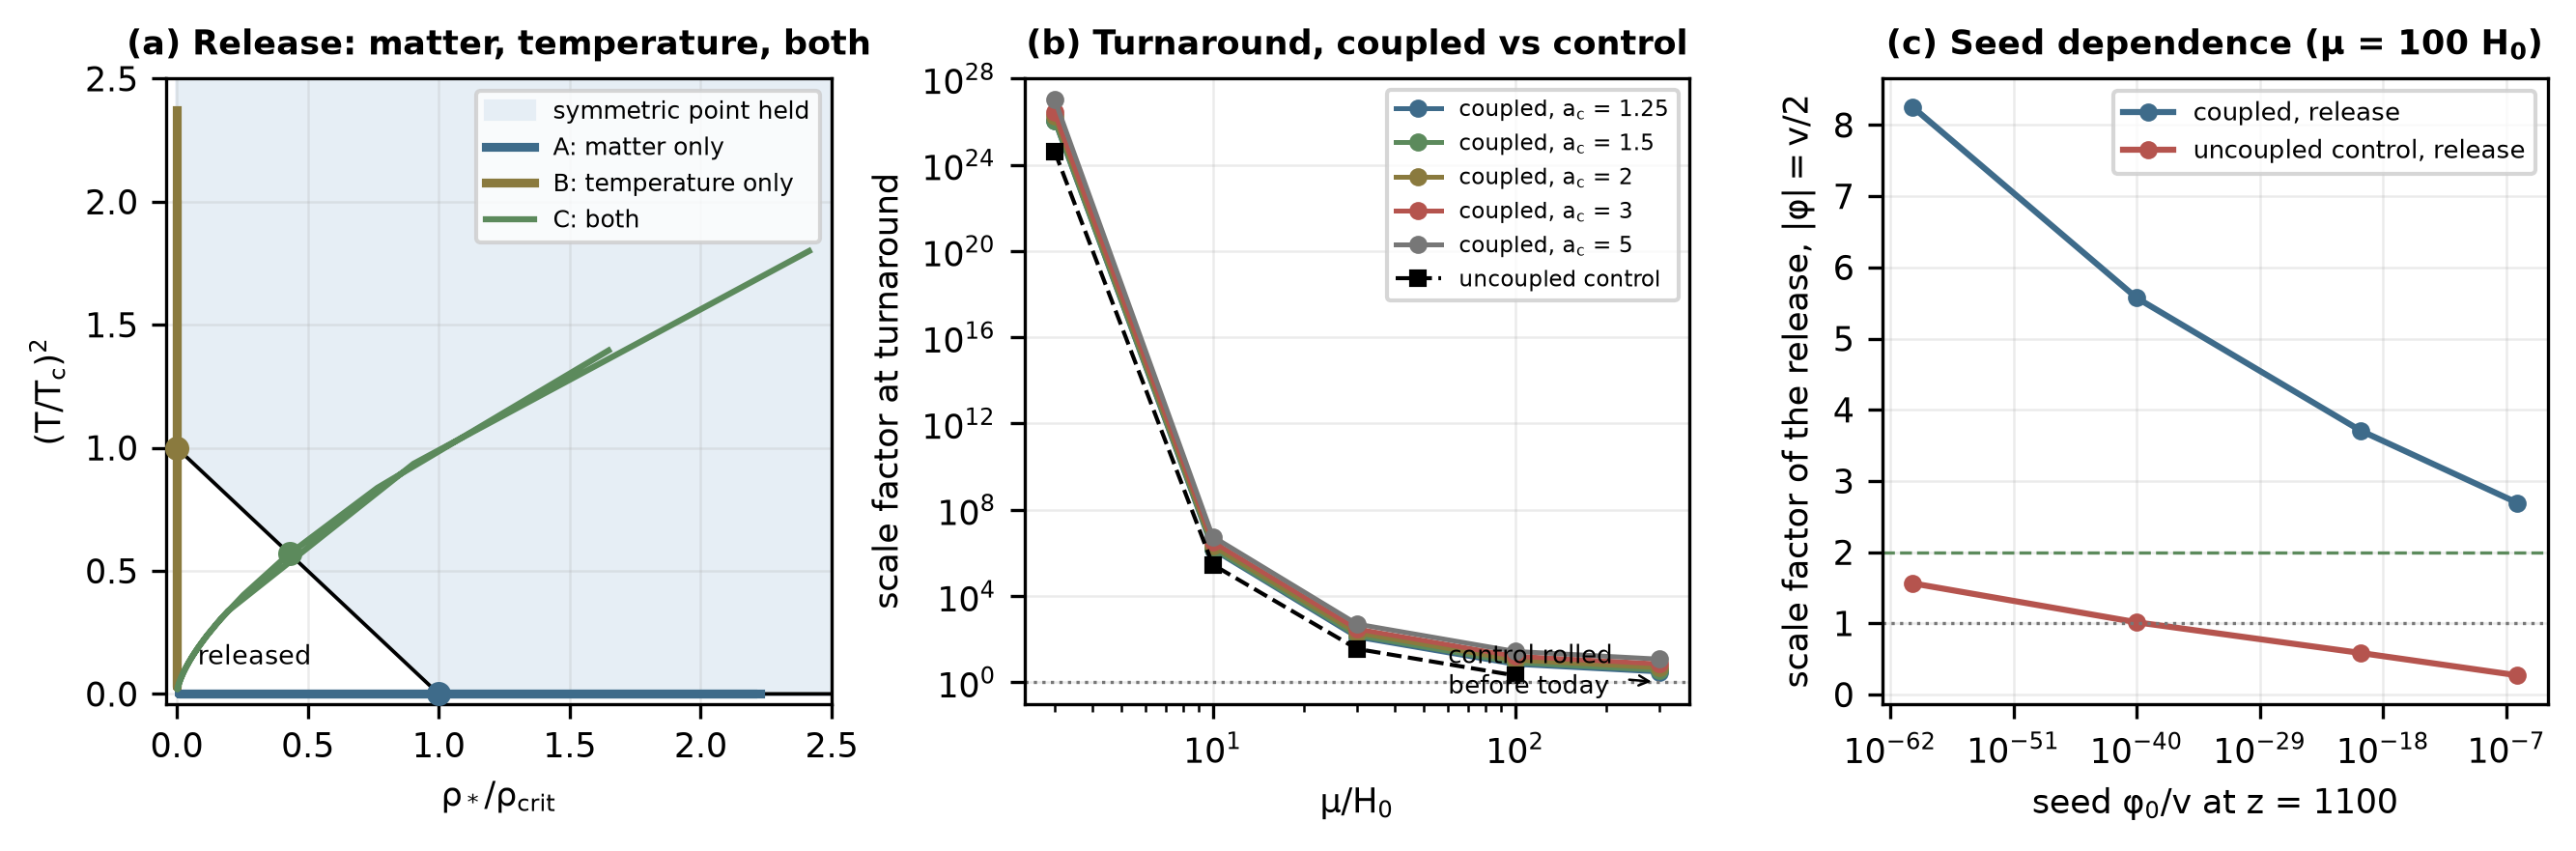
\includegraphics[width=1.00\textwidth]{../figures/fig14_release_scan.png}\caption{(a) The plane of matter density and temperature: the symmetric point is held above the line; trajectories of the matter-only, temperature-only and combined triggers (dots: release). (b) Scale factor at turnaround against $\mu$ for the coupled model at five $a_c$ and for the uncoupled control, which rolls before today at $\mu=300H_0$. (c) Scale factor of the release against the initial seed for the coupled model and the control.}\end{figure}
\subsection{Interventions on the turnaround}
Section 3.1 compared the coupled model with an uncoupled field. A sharper test intervenes on the cause itself (causal\_controls.py). Five models are evolved from today over the grid of Table 1: P, a positive cosmological constant (expands forever); N, a constant negative vacuum with matter (recollapses whatever the matter does, but decelerates today, $q_0=1.53$ for $q=1$, and is excluded by the observed acceleration); U, the scalar without the coupling; F, the coupled model with the matter density seen by the field frozen at its present value (an intervention on the field equation only, $do(\rho_*=\rho_{*,0})$; gravity still sees diluting matter); and D, the model of this paper. In all 100 grid points F stays held and expands forever, since $m_{\rm eff}^2=\mu^2(a_c^3-1)>0$, while D recollapses for every $q>0$ (75 of 75) and releases but keeps expanding for $q<0$ (there $V_0\ge-qV_c>0$, so $\rho>0$ and $H$ cannot vanish); U is never held: it rolls, or for $\mu=3H_0$, $q=10$ recollapses before reaching $v/2$ (Fig. 3). Within the model, the outcome changes from eternal expansion to recollapse when, and only because, the matter seen by the field is allowed to dilute. This does not make the coupling the only possible cause of a recollapse: a negative vacuum without it (N, U) also recollapses, but with a past that is not that of the observed universe over most of the range.

\begin{figure}[htbp]\centering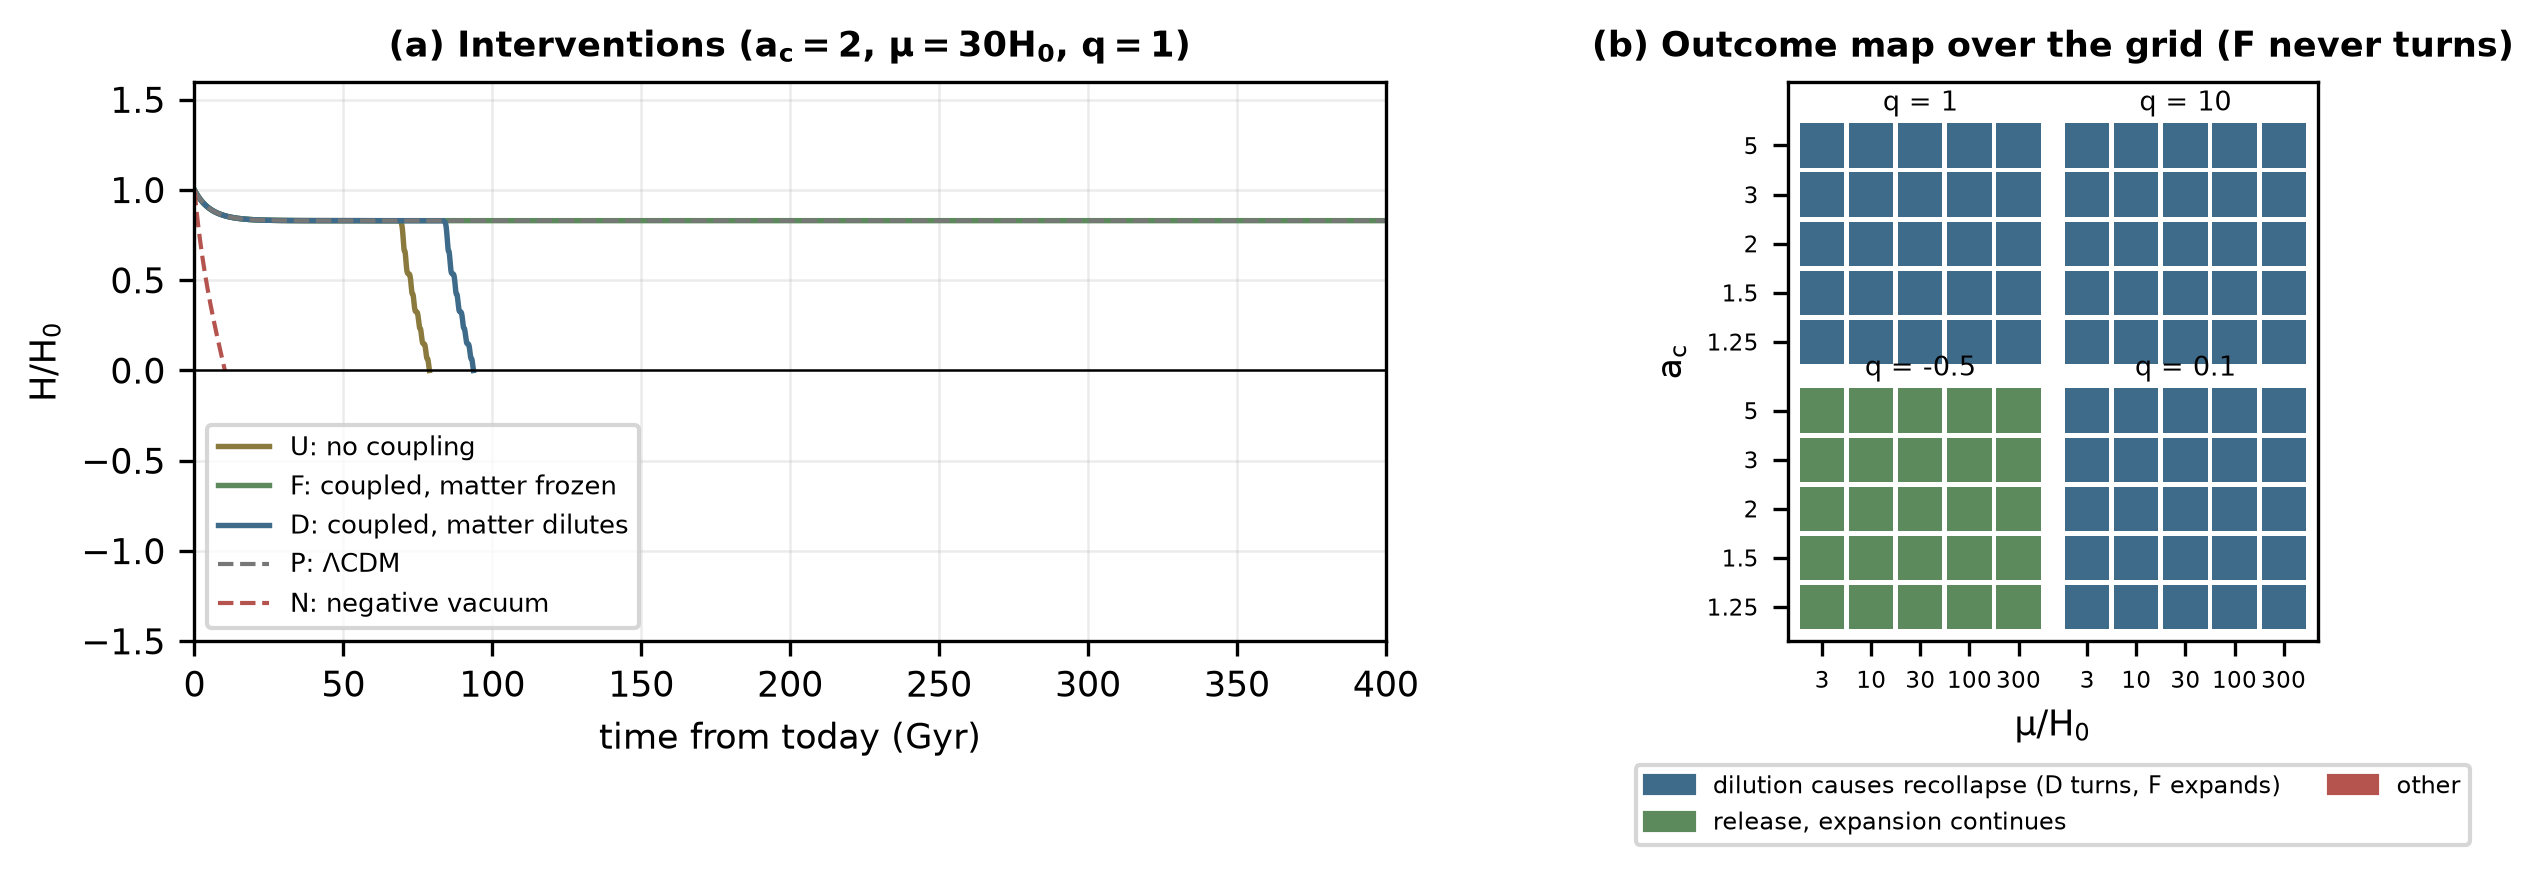
\includegraphics[width=1.00\textwidth]{../figures/fig19_causal_controls.png}\caption{Causal test. (a) $H(t)$ for the five models at $a_c=2$, $\mu=30H_0$, $q=1$: only D turns around after a $\Lambda$CDM past; F, identical except that the matter seen by the field does not dilute, expands forever. (b) Outcome over the grid of $a_c$, $\mu$ and $q$.}\end{figure}
\section{Contracting evolution and the effective bounce}
\subsection{The bounce prescription and why dissipation is needed}
A recollapse becomes a cycle only if the contraction reverses, which needs physics beyond general relativity. The effective loop-quantum-cosmology equations for a flat universe, for which they are derived [12, 13],

\begin{equation}
H^2=\frac{\rho}{3M_{\rm Pl}^2}\left(1-\frac{\rho}{\rho_c}\right),\qquad \dot H=-\frac{\rho+p}{2M_{\rm Pl}^2}\left(1-\frac{2\rho}{\rho_c}\right)
\end{equation}
are used as the bounce, with no curvature term appended. This is an assumption of the paper: the bounce is prescribed, not derived, and the physical $\rho_c\sim\rho_{\rm Pl}$ cannot be integrated, so $\rho_c$ is set far below it and the dependence on it is reported. A bounce alone is not enough. Without dissipation the contraction is dominated by the scalar's kinetic energy, which grows as $a^{-6}$, faster than radiation, and the bounce occurs at low density and is cold (cyclic\_extension.py): at $\rho_c=10^4V_c$ the cycles repeat with $G_n\simeq0.99$ but have no hot dense epoch, and they grow ($G_n\simeq1.19$ and $2.31$) at $\rho_c=10^5$ and $10^6V_c$, the cosmological hysteresis known from oscillating models [20]. Thermal dissipation, $\Upsilon=C_TT^3$, the form used for dissipative scalar dynamics in warm inflation [15], is negligible in the cold expanding universe and dominant in the hot contraction, where it turns the scalar's energy into radiation, so that the bounce is radiation dominated and hot. Sections 4.2--4.5 test the stability of repeated cycles, the contraction and the bounce; Section 5 follows the full cycle.

\subsection{Stability of repeated cycles}
Why dissipation is required can be isolated in the simplest homogeneous cycle: an open universe in a negative vacuum, $V=V_t+m^2\varphi^2/2$ with $V_t<0$, with radiation and the effective bounce (oscillation.py, oscillation\_validation.py). The hierarchy $\rho_c/|V_t|$ cannot be integrated at its physical value, so the cycles are simulated at $\rho_c/|V_t|=10^4$--$10^8$ in Planck units and the scaling of each quantity is measured. With radiation alone the cycles are exactly periodic: over 21 bounces the period varies by $2\times10^{-6}$, it scales as $|V_t|^{-0.500}$ and does not depend on $\rho_c$, and the trajectory is far from a sine (the fundamental harmonic carries 0.4\% of the power of $H$, and $\dot H>0$ only during $6.4\times10^{-4}$ of each cycle, at the bounce). Any oscillation of the scalar, however, is amplified from cycle to cycle: in the linear regime its energy grows by a factor between 6 and 396 per cycle, because the field is frozen near the bounce and released with a phase that does not return the energy it gained. Once it is no longer small, successive cycles grow, the cosmological hysteresis of oscillating models [20], and the growth obeys an energy-balance law: the continuity equation gives $\Delta(\rho a^3)=-W_n$ with $W_n=\oint p\,d(a^3)$, and at a turnaround $\rho a^3=-3a_{\max}$, so that $\Delta a_{\max,n}=W_n/3$, satisfied to $2\times10^{-3}$.

Dissipation into radiation competes with the amplification. The cycles run away for $\Upsilon P\le0.92$ and are stabilized for $\Upsilon P\ge3.1$, consistent with the criterion $\Upsilon P\gtrsim\ln\mu=2.33$ ($P$ the period, $\mu$ the energy multiplier). Over a grid of masses, dissipation strengths and initial amplitudes, 17 of 50 solutions are stable after 100 or more cycles and the rest grow; none shrinks and none loses its turnaround, and the stable ones remain stable over 1000 cycles, with $|G_n-1|\le3\times10^{-7}$ over the last 500 (Fig. 4). Stabilized cycles keep a constant entropy after a one-time increase; runaway cycles produce entropy without bound, which is the entropy problem of cyclic models [1, 18]. The instability does not depend on the bounce prescription (with $H^2=(\rho/3)[1-(\rho/\rho_c)^2]$ the multiplier is 5.4). Every cycle of this simple model has negative vacuum energy and therefore no epoch like ours; the matter-held vacuum of Section 2 is what supplies one, and the dissipation $\Upsilon=C_TT^3$ of Section 5 is what keeps its cycles on the stable side of this boundary.

\begin{figure}[htbp]\centering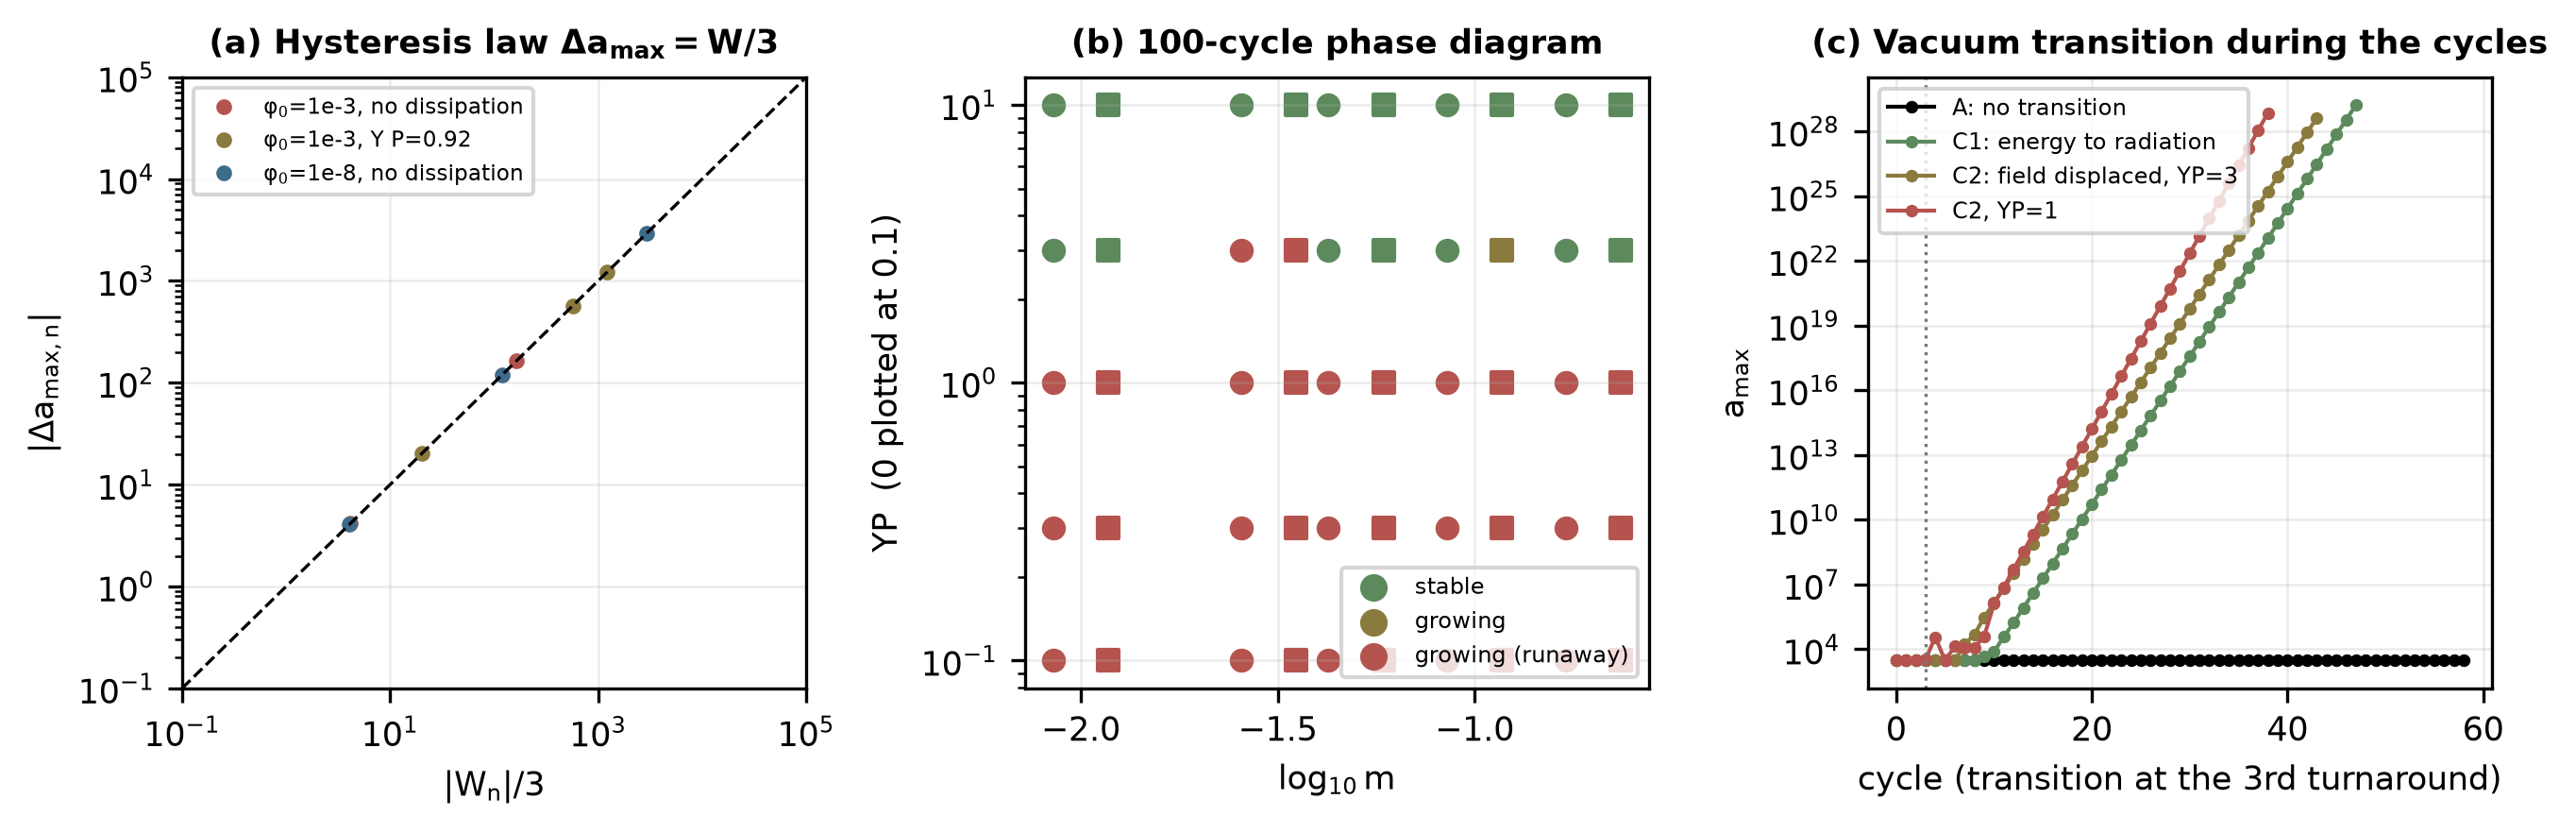
\includegraphics[width=1.00\textwidth]{../figures/fig12_hysteresis_stability.png}\caption{Stability of repeated cycles in a negative vacuum with an effective bounce. (a) Change of the turnaround radius against the pressure-volume loop $W_n/3$ for curvature-dominated cycles; dashed: the law $\Delta a_{\max}=W/3$. (b) Classification after 100 or more cycles over the scalar mass and the dissipation (circles $\varphi_0=10^{-8}$, squares $10^{-3}$): stable above $\Upsilon P\approx\ln\mu$. (c) A vacuum transition at the third turnaround turns a stable sequence into a growing one.}\end{figure}
\subsection{Anisotropy in the contraction}
A contracting universe is unstable to anisotropy: for Bianchi I the shear enters the Friedmann equation as $\rho_\sigma=\Sigma/a^6$, which grows relative to radiation as $a^{-2}$. In a single contraction from the turnaround to a bounce at $\rho_c$ the shear stays below 10\% of the density at the bounce only if it is below $s_{\max}=$$1.7\times10^{-27}$ of the matter density at the turnaround (contraction\_stability.py; the analytic scaling is reproduced to 7e-05). The cycles of Section 5 meet this condition in a way specific to them: the entropy produced in each cycle enlarges the next, so at a fixed temperature the scale factor is larger by $G_n$ and the shear, which is conserved in comoving terms, is diluted by $G_n^6$ per cycle. In the 100-cycle run the shear fraction at the bounce falls from $2\times10^{-16}$ to $1\times10^{-36}$ and then below $1\times10^{-300}$. This controls the shear inherited from the past, not shear generated anew in each cycle; for that the margin is the tolerance $s_{\max}$ itself.

An ekpyrotic phase widens the tolerance. A second scalar $\chi$ with $V_{\rm ek}=-V_ee^{-c\chi/M_{\rm Pl}}$, $c^2>6$, has $w=c^2/3-1>1$ and $\rho_\chi\propto a^{-c^2}$, so it dilutes the shear as $a^{c^2-6}$ [19, 22]. With its own dynamics, an exit and a decay into radiation after the exit, and starting with $\rho_\chi=10^{-12}\rho_m$ at the turnaround, $s_{\max}$ rises from $1.7\times10^{-27}$ to $1.7\times10^{-13}$ ($c=3$), $3.5\times10^{-13}$ ($c=5$) and $1.0\times10^{-11}$ ($c=7$), with 10.3, 7.6 and 3.9 e-folds of ekpyrotic contraction (Fig. 5). The tolerance is set by the onset: the ekpyrotic phase must dominate before the shear does. Ekpyrosis is not part of the cycle, which does not need it for the inherited shear; it is the mechanism the model would need if anisotropy were regenerated at the level $s>$$2\times10^{-27}$ each cycle.

\begin{figure}[htbp]\centering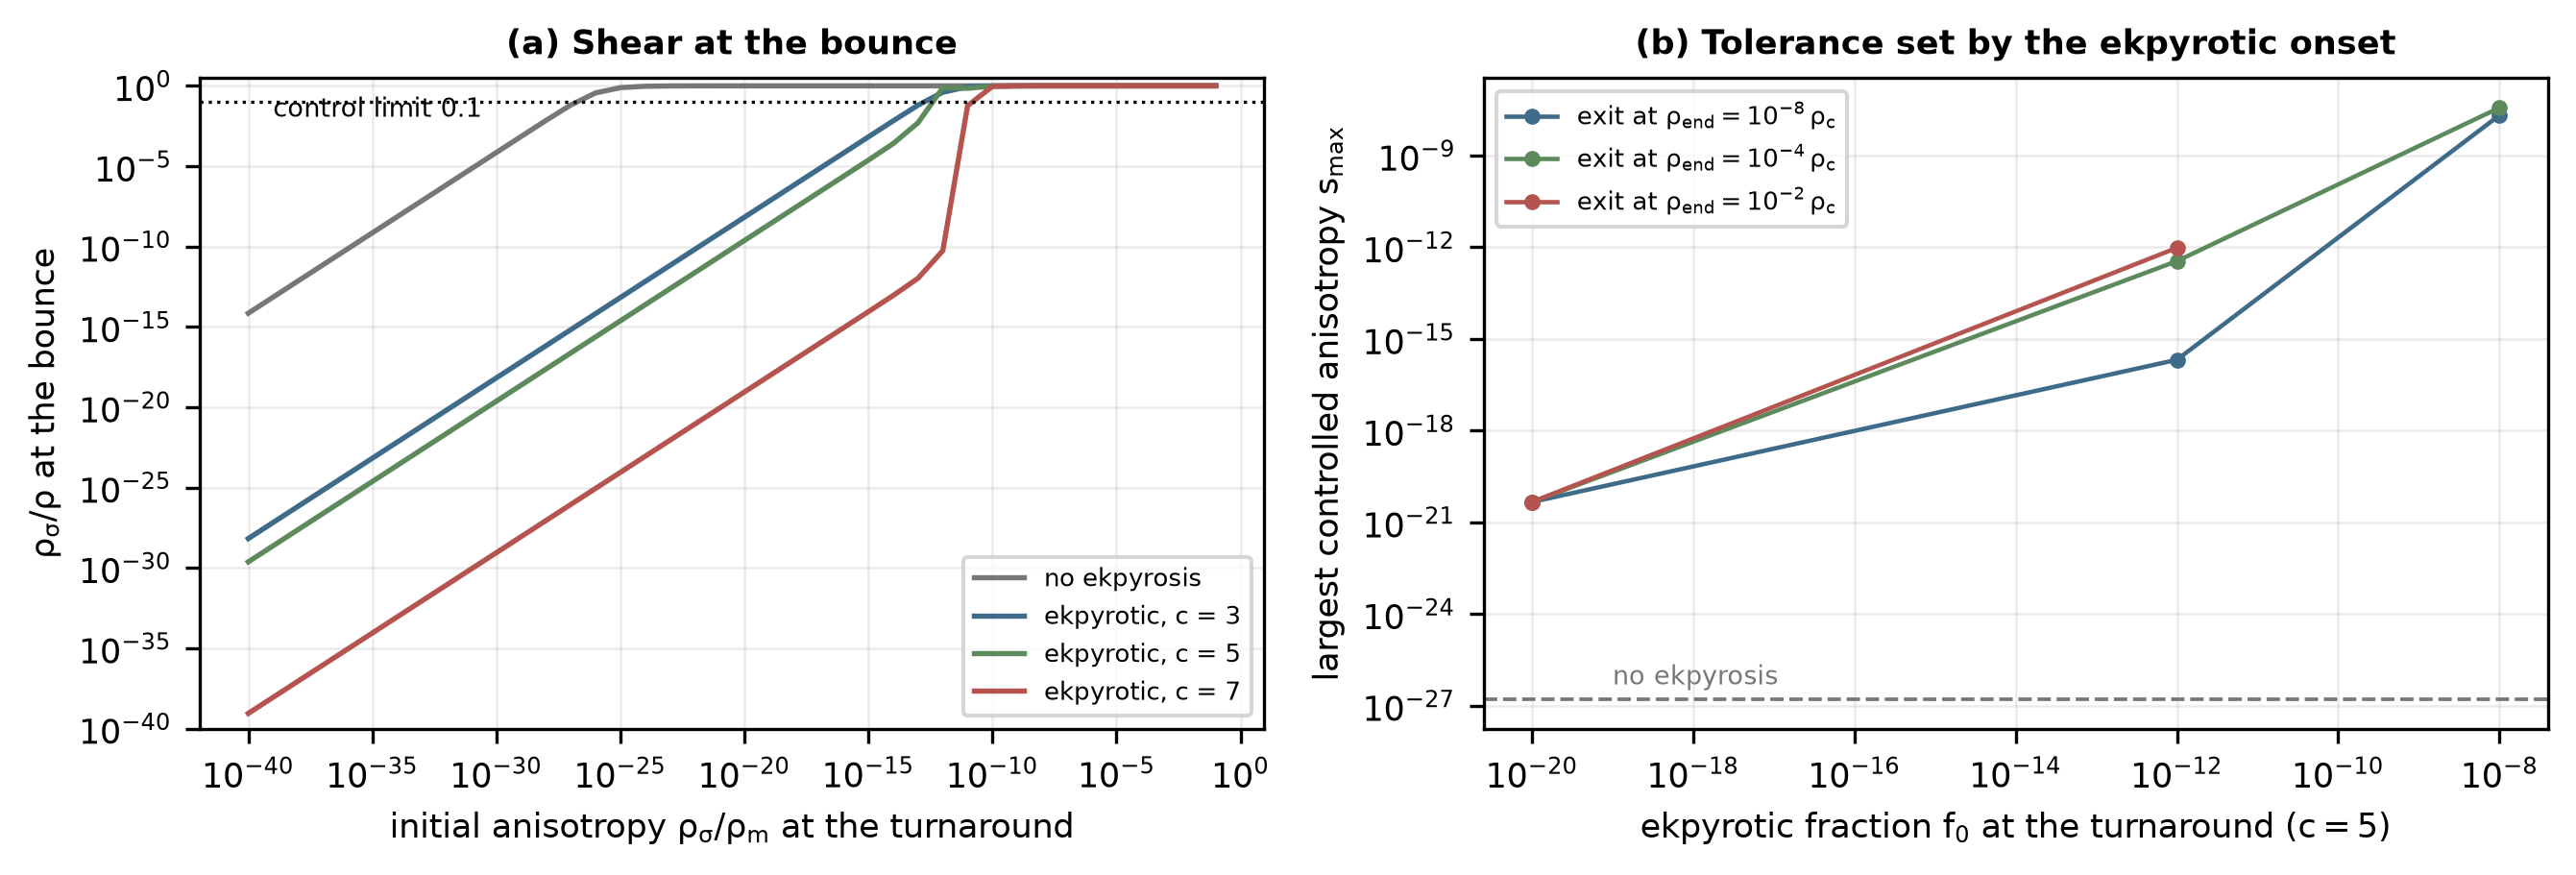
\includegraphics[width=1.00\textwidth]{../figures/fig20_contraction_stability.png}\caption{Shear in the contraction. (a) Shear fraction at the bounce against the anisotropy at the turnaround, without and with an ekpyrotic phase ($f_0=10^{-12}$, exit at $10^{-4}\rho_c$). (b) The largest controlled anisotropy against the ekpyrotic fraction at the turnaround, for three exit densities ($c=5$).}\end{figure}
\subsection{Bounce validation}
Three tests address the effective bounce (bounce\_validation.py). (A) Sensitivity to $\rho_c$: bounces at 1.83, 18.1, 172 MeV behave identically up to the bounce; the next cycle depends on $\rho_c$ only through rethermalization (next cycle: 1.83 MeV: empty; 18.1 MeV: working; 172 MeV: working). (B) The effective equations through the bounce: without projection inside $\rho>0.4\rho_c$ the constraint holds to $6\times10^{-6}$, $d\ln\rho/d\ln a=-3(1+w)$ to $2\times10^{-7}$, the density and the entropy are continuous across the bounce, and the curvature invariants are finite, $R=4.0000\rho_c$ and $K=5.3332\rho_c^2$ at the bounce against the analytic $3(\rho+p)=4\rho_c$ and $16\rho_c^2/3$ for radiation. (C) An independent bounce: general relativity with a negative-energy stiff fluid $\rho_g=-g/a^6$ in place of the LQC correction. Its bounce density is set by a comoving constant, so it is not fixed from cycle to cycle, and the bounce temperature is 2.72e+03 MeV in successive cycles, against 172, 172, 172, 172, 172 MeV for the LQC bounce. The cycle survives the change of mechanism, but its self-similarity is a property of a bounce at a fixed density, not of bounces in general (Fig. 6).

\begin{figure}[htbp]\centering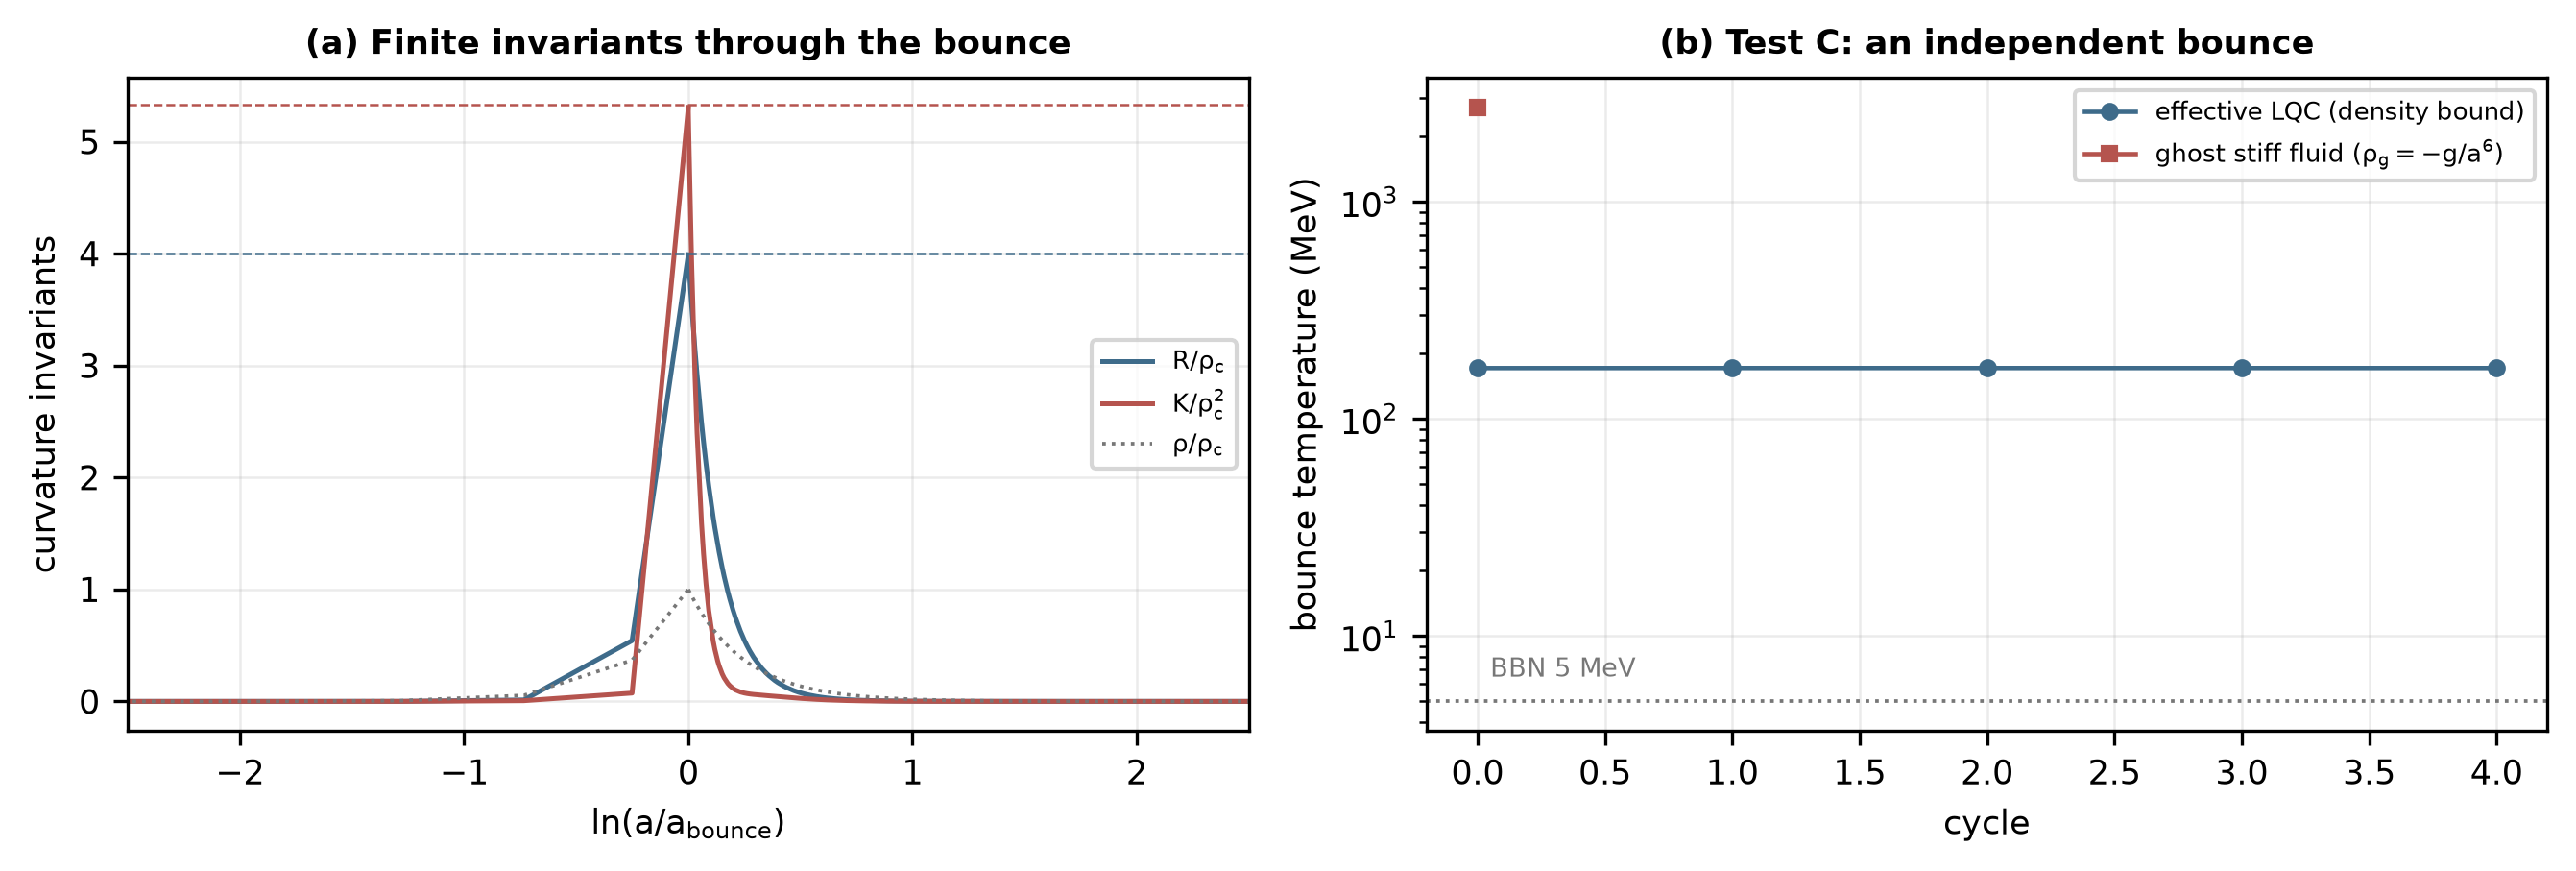
\includegraphics[width=1.00\textwidth]{../figures/fig21_bounce_validation.png}\caption{Bounce validation. (a) Curvature invariants and density through the first bounce of the baseline run; dashed lines: the analytic bounce values for radiation. (b) Test C: bounce temperature per cycle for the LQC bounce and for a ghost stiff fluid.}\end{figure}
\subsection{Black holes through the bounce}
The black holes of a cycle do not take part in its rethermalization. Their mass function $n(M,t)$ is evolved through the contraction (compact\_relics.py) with $\partial_tn+3Hn+\partial_M(\dot Mn)=C_{\rm merge}+S_{\rm form}$: accretion of radiation $\dot M=27\pi G^2M^2\rho_r$ [23], capped at the Hubble mass; binned mergers with the capture cross-section; and the present population as the source (stellar remnants with $\Omega=10^{-4}$ near $10\,M_\odot$, supermassive holes with $\Omega=7.6\times10^{-6}$ near $10^8M_\odot$, with exponential cut-offs above 100 and $5\times10^9M_\odot$). The quantity that decides whether a homogeneous bounce is possible is the fraction of space inside horizons, $f_V$. At the bounce ($T_b=172$ MeV) it is $2\times10^{-4}$ for the present population and $5\times10^{-4}$ with accretion and mergers (Fig. 7a). Holes above $5\,M_\odot$ accrete runaway to the Hubble mass, and since $f_V\propto T^3$ the evolved population would reach $f_V=1$ for a bounce above approximately 2.2 GeV; all supermassive mass in holes of a single mass gives 539, 2.5e+03, 1.16e+04 MeV for $10^{10}$, $10^9$ and $10^8M_\odot$. The black holes therefore bound the bounce from above, while BBN bounds it from below: $5\ \mathrm{MeV}\lesssim T_b\lesssim2.2$ GeV within this prescription, or $\lesssim0.5$ GeV for the single-mass estimate. The surviving holes enter the next cycle as relics, and their number per unit entropy falls by $G_n^3$ per cycle.

This upper limit is an estimate within the stated population prescription, not a general cosmological bound, and its sensitivity was tested (relic\_sensitivity.py, Table S9). Adding horizon volumes treats the holes as nonoverlapping; for randomly placed, overlapping spheres the occupied fraction is $1-e^{-f_V}$ and continuum percolation sets in at $f_V\approx0.34$, which lowers the bound from 2.17 to 1.52 GeV. Changing the stellar abundance threefold either way leaves it unchanged; the supermassive abundance, cut-off and characteristic mass move it between 1.02 and 3.14 GeV (between 0.71 and 2.19 GeV with the overlap threshold); without accretion and mergers it is 3.00 GeV, and without mergers alone it is unchanged. Accretion is the sensitive input. With two and three times the geometric capture rate the bound falls to 1.71 and 1.18 GeV, and with ten times to 29 MeV, below the baseline bounce, because the mass above which holes grow to the Hubble mass falls with the rate. The geometric capture cross-section is the physical rate for radiation, and Bondi accretion of a relativistic fluid is of the same order, so the baseline is the physical choice, but the bound inherits that assumption. Clustering lowers it locally: the supermassive holes trace galaxies, and a region overdense by $1+\delta$ reaches the threshold at a temperature lower by $(1+\delta)^{-1/3}$, 0.33 GeV for $\delta=100$. A strongly inhomogeneous contraction, in which horizon volumes cannot be treated as a dilute gas at all, is outside this estimate. Within these assumptions the window is approximately 5 MeV to 0.7--3.1 GeV, and the baseline bounce at 172 MeV lies inside it for every variant except the tenfold accretion. Closing the window at the overlap threshold, at the lowest population variant or at the clustered estimate lowers the joint viability of Section 6.3 from 6.8\% to 5.7\%, 3.9\% and 2.5\%.

\begin{figure}[htbp]\centering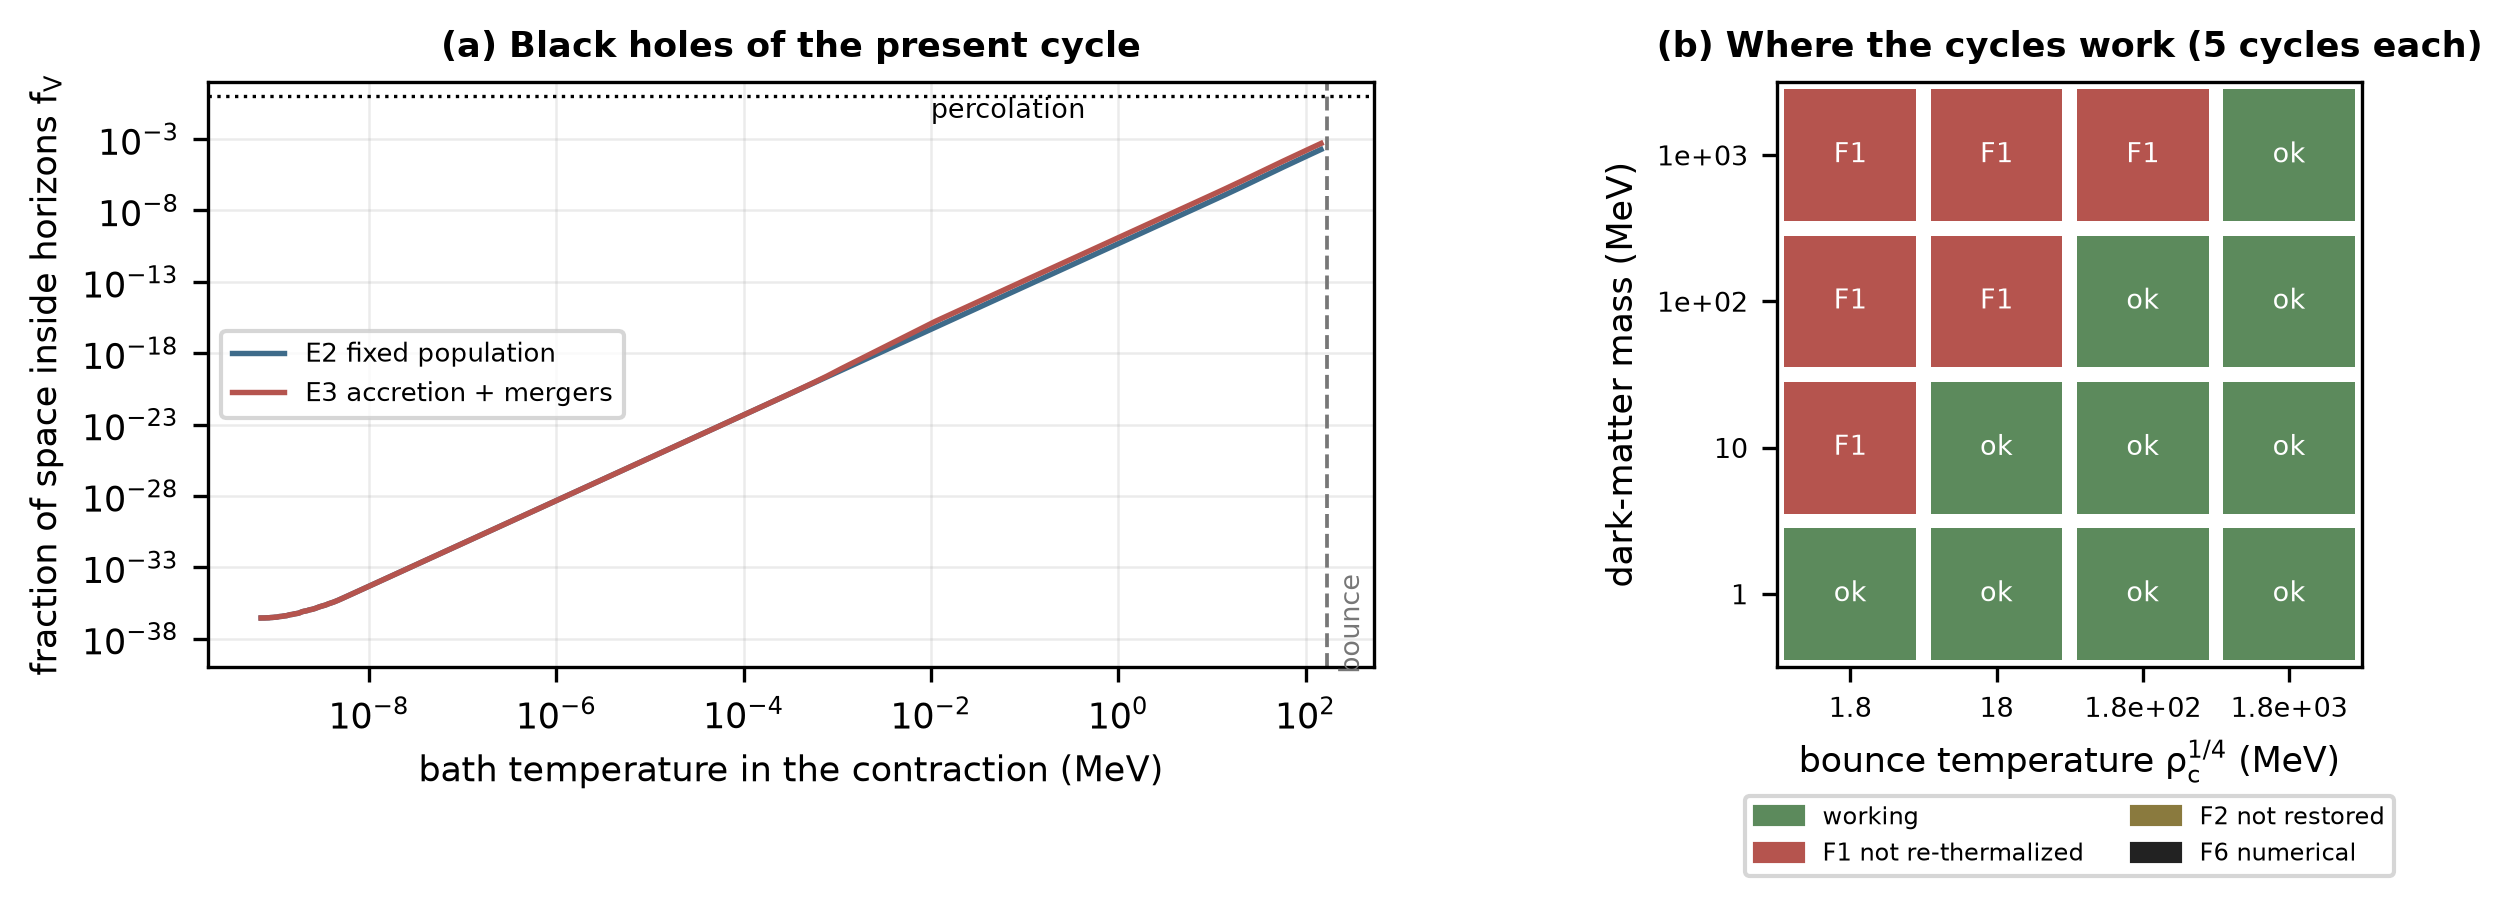
\includegraphics[width=1.00\textwidth]{../figures/fig22_relics_failure_map.png}\caption{(a) Fraction of space inside black-hole horizons through the contraction, for the present population (E2) and with accretion and mergers (E3). (b) Outcome of five continuous cycles over dark-matter mass and bounce temperature: the cycles work where the bounce rethermalizes the dark matter (Section 6.2).}\end{figure}
\subsection{Physical status of the low-density bounce}
The bounce used in this paper is a phenomenological prescription, and its status should be stated plainly. Loop quantum cosmology derives the effective equations of Section 4.1 for a bounce at $\rho_c\approx0.41\rho_{\rm Pl}$ [12, 13]. The simulations place it instead at $\rho_c=10^{44}H_0^2M_{\rm Pl}^2$, a bounce temperature of approximately 172 MeV, some twenty orders of magnitude below the Planck temperature and some eighty below the Planck density. At that density standard loop quantum cosmology predicts no bounce, and no established theory predicts one. The quadratic form $H^2=(\rho/3)(1-\rho/\rho_c)$ is used because it is the simplest modification of the Friedmann equation that is nonsingular, conserves stress-energy and fixes the bounce at a density; the instability of repeated cycles does not depend on this form (Section 4.2). The ghost-fluid bounce of Section 4.4 is a sensitivity test, not a physical proposal: a negative-energy stiff fluid violates the null energy condition and is not known to be a healthy field theory.

What the simulations establish is therefore conditional. If some mechanism reverses the contraction at a fixed density between the BBN and black-hole bounds, the cycle of Section 5 follows from the remaining equations, and the properties that depend on the bounce are isolated: the bounce temperature is set by $\rho_c$; the next cycle depends on $\rho_c$ only through the rethermalization of the dark matter (Section 4.4); and self-similar cycles need a bounce at a fixed density, which a ghost-fluid bounce does not provide. The simulations are not a derivation of a realistic quantum-gravity bounce, and none of the results should be read as evidence that such a bounce occurs.

\section{Reheating, dark matter and repeated cycles}
\subsection{Continuous reheating without resets}
The cycle is followed with no variable reset (continuous\_cycles.py). The dark matter is a thermal species with its own Boltzmann equation [16, 17]; its particles have the field-dependent mass $m_{\rm eff}=mA(\varphi)$ and are in kinetic equilibrium with the bath, so that their comoving number $N=na^3$ and their energy per particle follow

\begin{equation}\begin{gathered}
\dot N=-\langle\sigma v\rangle\frac{N^2-N_{\rm eq}^2}{a^3},\qquad n_{\rm eq}=c_n\frac{x^2K_2(x)}{2}T^3,\\
\epsilon=m_{\rm eff}\frac{K_1(x)}{K_2(x)}+3T,\qquad x=\frac{m_{\rm eff}}{T}
\end{gathered}\end{equation}
The scalar exchanges energy with the bath through the dissipation and through the field dependence of the particle masses:

\begin{equation}\begin{gathered}
\ddot\varphi+(3H+\Upsilon)\dot\varphi+V_0'+F=0,\qquad F=n\frac{K_1}{K_2}mA'(\varphi),\\
\dot\rho_{\rm th}=-3H(\rho_{\rm th}+p_{\rm th})+\Upsilon\dot\varphi^2+F\dot\varphi
\end{gathered}\end{equation}
with $\rho_{\rm th}=\rho_r+n\epsilon$, $p_{\rm th}=\rho_r/3+nT$ and $\Upsilon=C_TT^3$; the temperature is a state variable and the total stress-energy is conserved by construction. The single coupling $A(\varphi)$ produces both the hot-phase thermal mass (a relativistic gas gives $F\simeq nm_{\rm eff}mA'/2T$) and the late hold (a cold gas gives $F=\rho_*A'$), so the restoration of the vacuum and the freeze-out of the dark matter are outputs. In physical units $T=1$ is 1.82 meV, $C_T=1$ is a dissipation $T^3/f^2$ with $f=(H_0M_{\rm Pl}^3)^{1/4}=2.1$ TeV, and $\langle\sigma v\rangle$ is fixed once, by requiring the present dark-matter density in the held epoch of the repeating cycle ($8.0\times10^{-28}$ cm$^3$ s$^{-1}$ for $m=10.1$ MeV). This is 0.0147 times its value for freeze-out at constant mass, because in the cycle the dark matter freezes out while the field is still displaced and the dark matter heavier. Two numerical devices are used and tested in Section 6.1: where the dissipation exceeds every other rate by $10^3$ the field moves at its terminal velocity, and $H$ is projected onto the constraint once per doubling of the scale factor away from the turning points; relative to the density the constraint residual stays below $5\times10^{-6}$ throughout.

The first result is negative. With $m=10.1$ MeV and a bounce at 1.8 MeV, our cycle completes (release, turnaround at $\ln a=3.13$, a radiation-dominated bounce) but the next cycle is empty: the dark matter reaches the bounce with $x=m_{\rm eff}/T=55$, is annihilated during the hot contraction and is not regenerated ($Y/\kappa=1.8\times10^{-6}$ in the next cycle), the field is frozen at $|\varphi|=0.96v$ by the overdamping, and there is no matter era (peak matter fraction 0.005) and no dark-energy epoch. Prescribed resets of the dark-matter abundance at freeze-out, used in an earlier version of this model, hide exactly this failure.

The second result is that the same equations give working cycles once the bounce rethermalizes the dark matter, $T_b\gtrsim m_{\rm eff}/5$. With $m=10.1$ MeV, a bounce at 172 MeV and today's anisotropy set to $\Omega_\sigma=10^{-30}$, 100 cycles were integrated with no reset of any variable (Fig. 8, Table 2). In every cycle the field is frozen at the bounce at $|\varphi|/v=0.38\pm0.00$, the dark matter returns to equilibrium ($x_b=0.6$--$0.7$) and freezes out while the field is still displaced (yield $Y_{\rm fo}/\kappa=61.52\pm0.04$); the field is then restored, which lowers the dark-matter mass and heats the bath, and the held epoch has $Y/\kappa=1.01\pm0.02$; the field is damped toward $\varphi=0$ by 61--62 orders of magnitude, a matter era follows (peak matter fraction $1.00\pm0.00$), then a dark-energy epoch with the field held ($5.28\pm0.01$ e-folds of accelerated expansion), a release, a turnaround and the next bounce. The held e-folds vary between 5.27 and 5.39, because the value at which the field freezes depends on the phase of its oscillation when the overdamping sets in (Section 5.2). The growth per cycle, $\ln G_n=7.66\pm0.00$, equals the entropy growth $\frac{1}{3}\ln(S_{n+1}/S_n)$ to within $1\times10^{-2}$ in every cycle: the second law holds and is absorbed by Tolman's growing cycles [1].

A second run of 100 cycles with $m=100$ MeV and the same bounce (continuous\_cycles\_100MeV.json) works as well: held e-folds $4.26\pm0.05$, peak matter fraction $0.96\pm0.00$, $\ln G_n=5.49\pm0.04$, with the field freezing at $\varphi_b=0.28\pm0.01v$. That point is marginal: it lies on the working branch of Section 6.2 only because the field freezes far from $v$, and one-at-a-time changes of $\mu$, $q$ or $C_T$ move it to the empty branch.

An earlier version of this model prescribed three steps that the present equations produce themselves: the dark-matter abundance was reset at freeze-out, the hot-phase restoration of the vacuum was applied through its adiabatic result, and the dissipation was capped (hot\_cycles.py). That version gives exactly self-similar cycles with $G_n=231.8=(S_{n+1}/S_n)^{1/3}$ and 3.63 held e-folds, and its controls fail as expected (without the freeze-out reset no matter era remains; without dissipation the bounce is cold and kinetic dominated). The continuous cycles reproduce its qualitative structure, and in addition expose the failure that the resets hid (the cold bounce above) and the cycle-to-cycle variation of the held epoch explained in Section 5.2.

\begin{table}[htbp]\centering\footnotesize\setlength{\tabcolsep}{3pt}
\caption{Continuous cycles without resets (baseline: $m=10.1$ MeV, $\rho_c^{1/4}$ = 172 MeV, $C_T=1$, $a_c=2$, $\mu=30H_0$, $q=1$, $\Omega_{\sigma,0}=10^{-30}$). Cycle 0 starts today; $x_b$ and $\varphi_b$ at the bounce that ends the cycle; $Y/\kappa$ the dark matter relative to the present value; the last row is cycle 99. All cycles: continuous\_cycles.csv.}
\begin{tabular}{llllllllll}
\toprule
cycle & $T_b$ (MeV) & $x_b$ & $\varphi_b/v$ & $Y_{\rm fo}/\kappa$ & $Y/\kappa$ held & peak matter & held e-folds & $\ln G_n$ & $\frac13\ln\frac{S_{n+1}}{S_n}$ \\ \midrule
0 & 172 & 0.6 & 0.357 & (today) & (today) & 0.311 & 2.84 & 7.78 & 7.76 \\
1 & 172 & 0.7 & 0.378 & 61.20 & 1.160 & 0.996 & 5.39 & 7.66 & 7.67 \\
2 & 172 & 0.6 & 0.375 & 61.80 & 0.989 & 0.995 & 5.29 & 7.67 & 7.66 \\
3 & 172 & 0.6 & 0.376 & 61.52 & 1.013 & 0.995 & 5.27 & 7.66 & 7.67 \\
4 & 172 & 0.6 & 0.375 & 61.53 & 1.007 & 0.995 & 5.29 & 7.66 & 7.66 \\
5 & 172 & 0.6 & 0.376 & 61.52 & 1.011 & 0.995 & 5.29 & 7.66 & 7.67 \\
6 & 172 & 0.6 & 0.375 & 61.52 & 1.007 & 0.995 & 5.27 & 7.66 & 7.66 \\
7 & 172 & 0.6 & 0.376 & 61.52 & 1.011 & 0.995 & 5.29 & 7.66 & 7.67 \\
99 & 172 & 0.6 & 0.376 & 61.52 & 1.011 & 0.995 & 5.29 & 7.66 & 7.67 \\
\bottomrule
\end{tabular}
\end{table}
\begin{figure}[htbp]\centering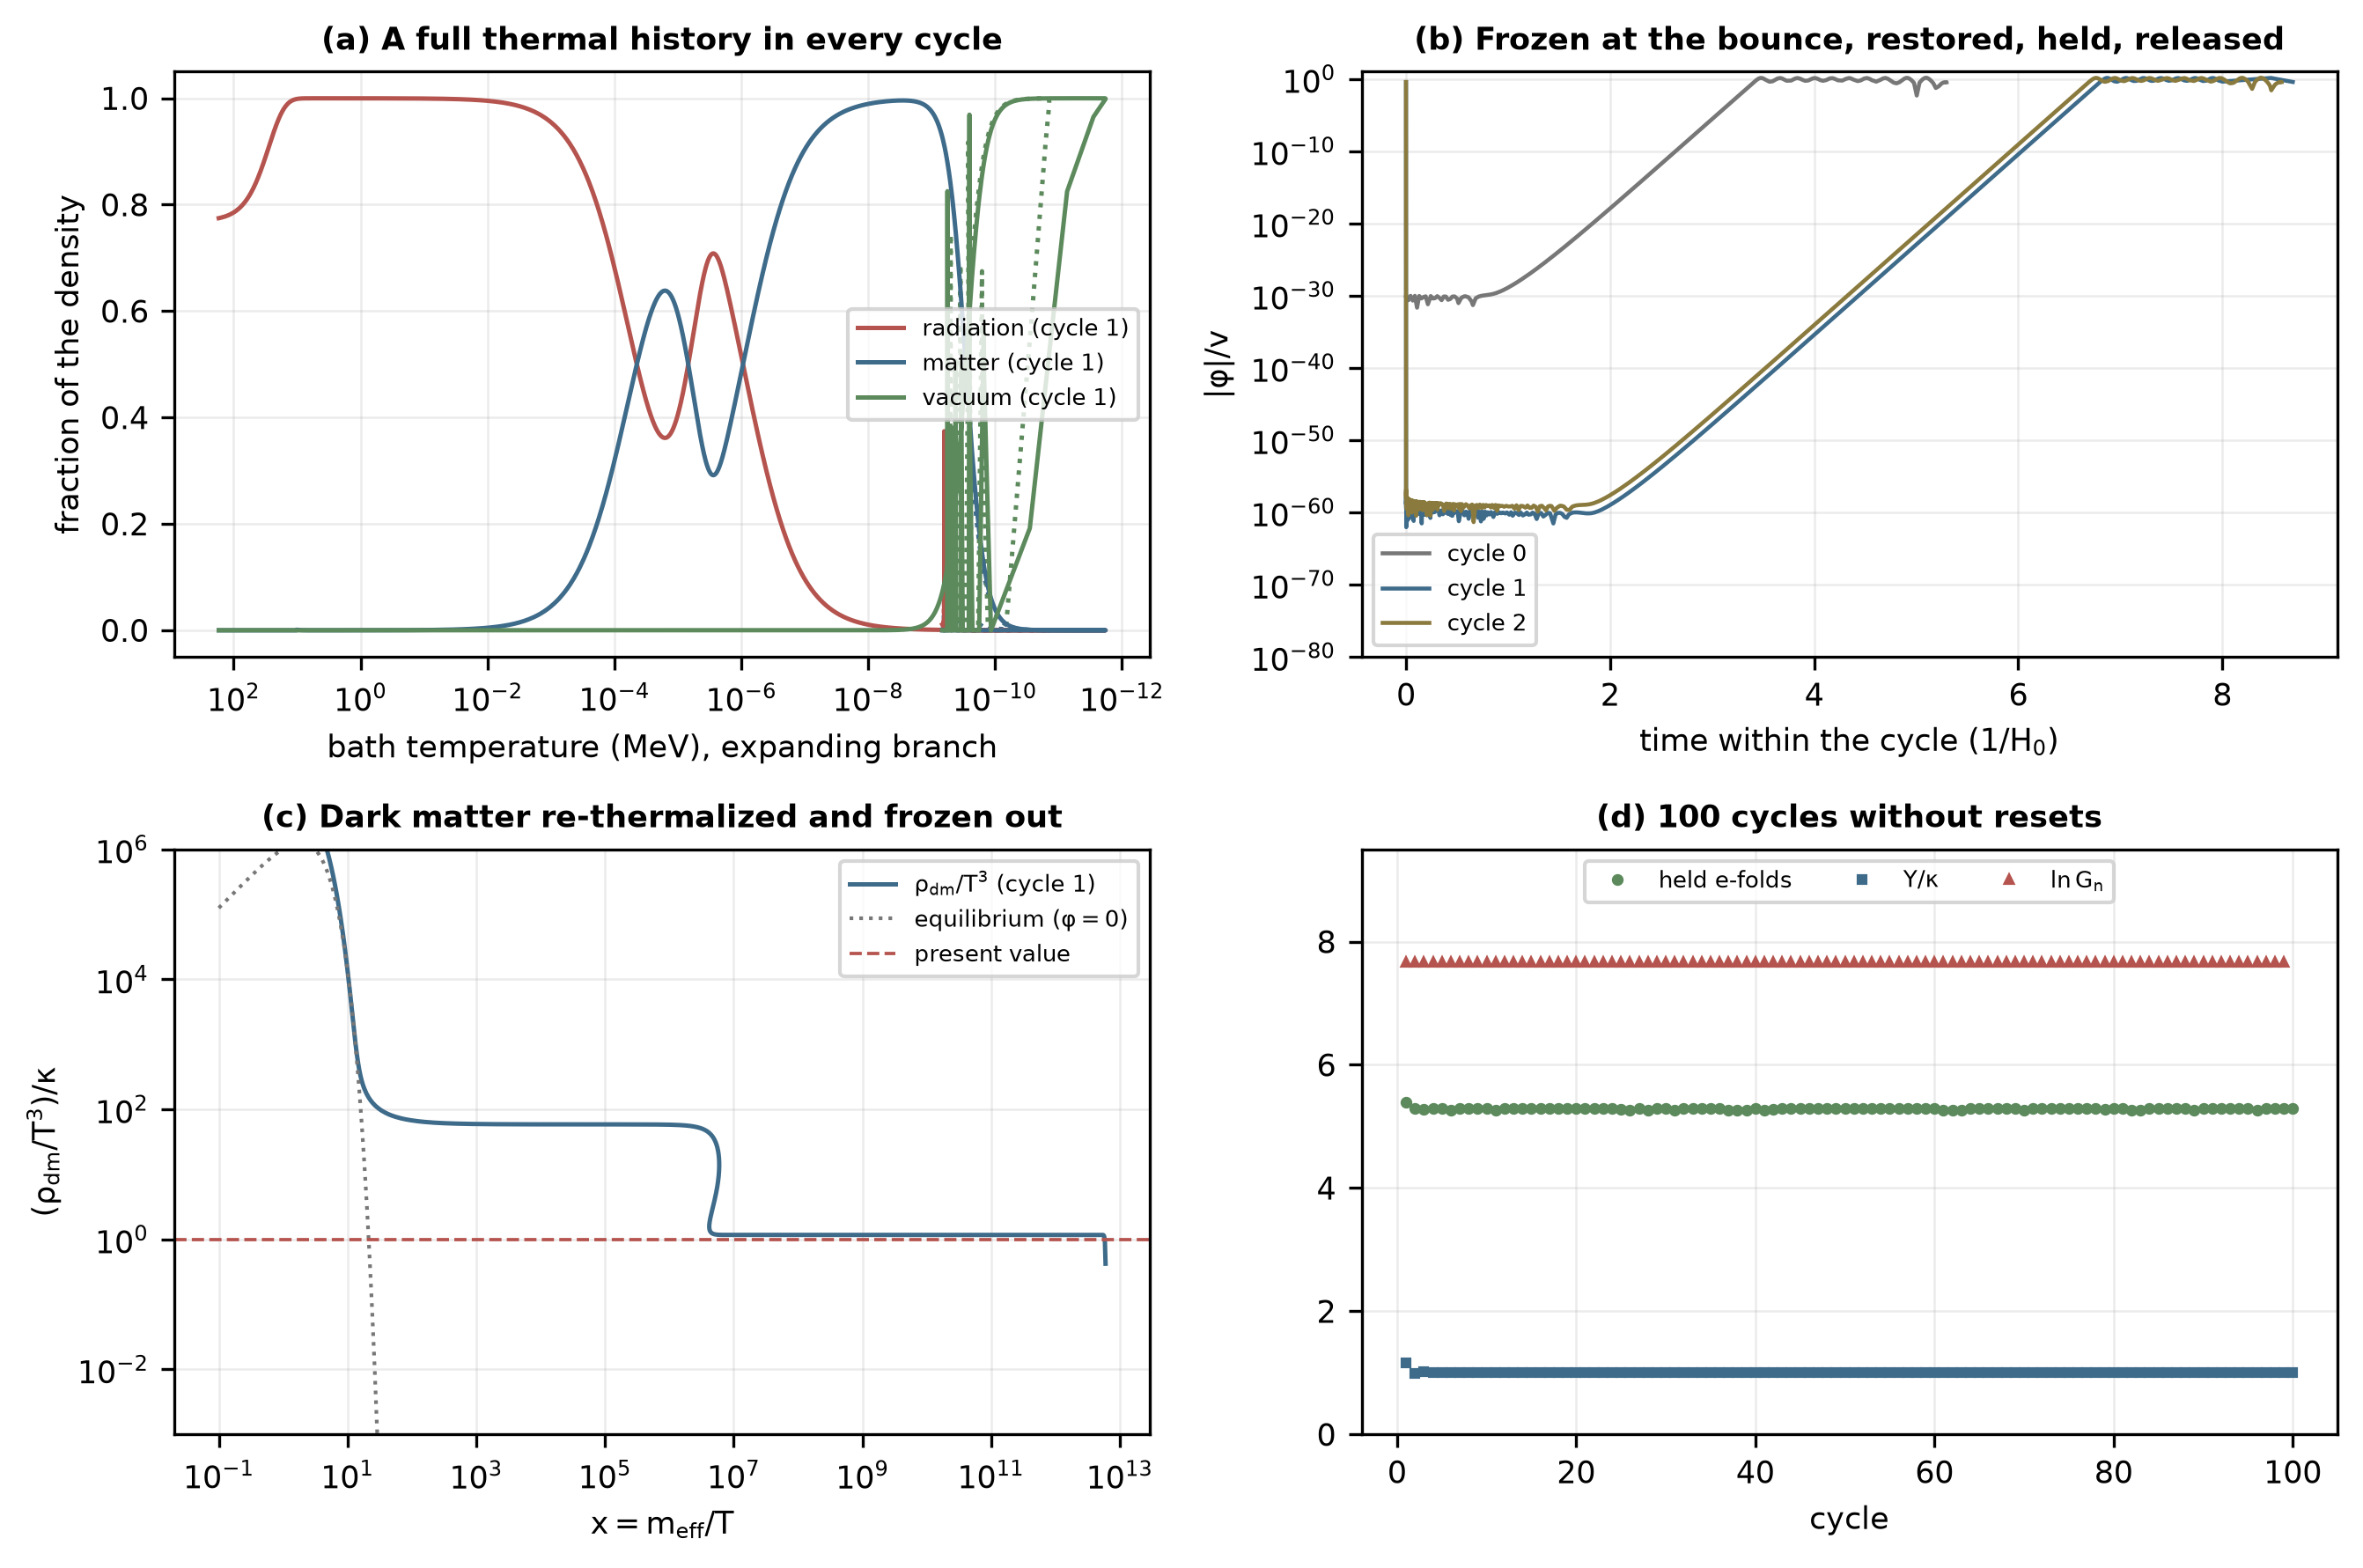
\includegraphics[width=1.00\textwidth]{../figures/fig17_continuous_cycles.png}\caption{Continuous cycles without resets. (a) Fractions of radiation, matter and vacuum energy against the bath temperature in the expanding branch, for today's cycle (dotted, from today) and the next (solid). (b) The field in three cycles: frozen at the bounce, released from the hot phase, damped to $\varphi\approx0$, held by the matter and released. (c) The dark matter of cycle 1 against $x=m_{\rm eff}/T$: in equilibrium at the bounce, frozen out while the field is displaced (upper plateau), and reduced to the present ratio when the restoration lowers its mass and heats the bath (lower plateau). (d) Held e-folds, $Y/\kappa$ and $\ln G_n$ over 100 cycles.}\end{figure}
\subsection{The cycle as an attracting fixed point}
Why the cycle repeats can be stated as a property of a map. At a bounce the density is fixed at $\rho_c$, the field is overdamped with its velocity slaved, and the remaining freedom is the value $\varphi_b$ at which the field is frozen. The bounce-to-bounce map $\varphi_{b,n}\mapsto\varphi_{b,n+1}$ was probed by starting one cycle from the baseline bounce state with $\varphi_b$ set to each of 15 values between $0.02v$ and $v$ and integrating to the next bounce (cycle\_map.py, Fig. 9a). For $m=10$ MeV every start gives a working cycle, the map has a single fixed point at $\varphi_b^*=0.376v$, and its slope there is $-0.14$: a deviation shrinks by a factor of approximately 7 in one cycle, so the repeating cycle is an attracting fixed point whose basin covers the whole interval tested. For $m=100$ MeV the fixed point lies at $0.283v$ with slope $-0.69$: still attracting, with oscillating and slower convergence. The empty branch of Section 6.2 is not a second fixed point of this map; it is reached when the dark matter is not regenerated at the bounce, a second state variable that the one-dimensional map holds fixed.

The held epoch itself has a closed form. Acceleration begins when the matter density falls to $2V_c$ and the field is released when it falls to $\rho_{\rm crit}$, which takes $\frac13\ln(2V_c/\rho_{\rm crit})$ e-folds; the tachyonic field then needs $N_{\rm grow}$ more e-folds to grow from its restored value $\varphi_{\rm rest}$ to $0.1v$,

\begin{equation}\begin{gathered}
N_{\rm held}=\frac{1}{3}\ln\frac{2V_c}{\rho_{\rm crit}}+N_{\rm grow},\qquad \int_0^{N_{\rm grow}}\frac{\lambda(N)}{H_\Lambda}\,dN=\ln\frac{0.1\,v}{\varphi_{\rm rest}},\\
\lambda=\Big(\mu^2\big(1-e^{-3N}\big)+\tfrac94H_\Lambda^2\Big)^{1/2}-\tfrac32H_\Lambda
\end{gathered}\end{equation}
with $H_\Lambda=(V_c/3)^{1/2}$. With $\varphi_{\rm rest}$ read from each cycle of the 100-cycle run, this reproduces the integrated held e-folds to 0.020 e-folds (rms over 100 cycles; largest deviation 0.067; Fig. 9b). The variation of the held epoch between cycles is therefore explained: it is the logarithm of how deeply each cycle restored the field, divided by the tachyonic growth rate.

\begin{figure}[htbp]\centering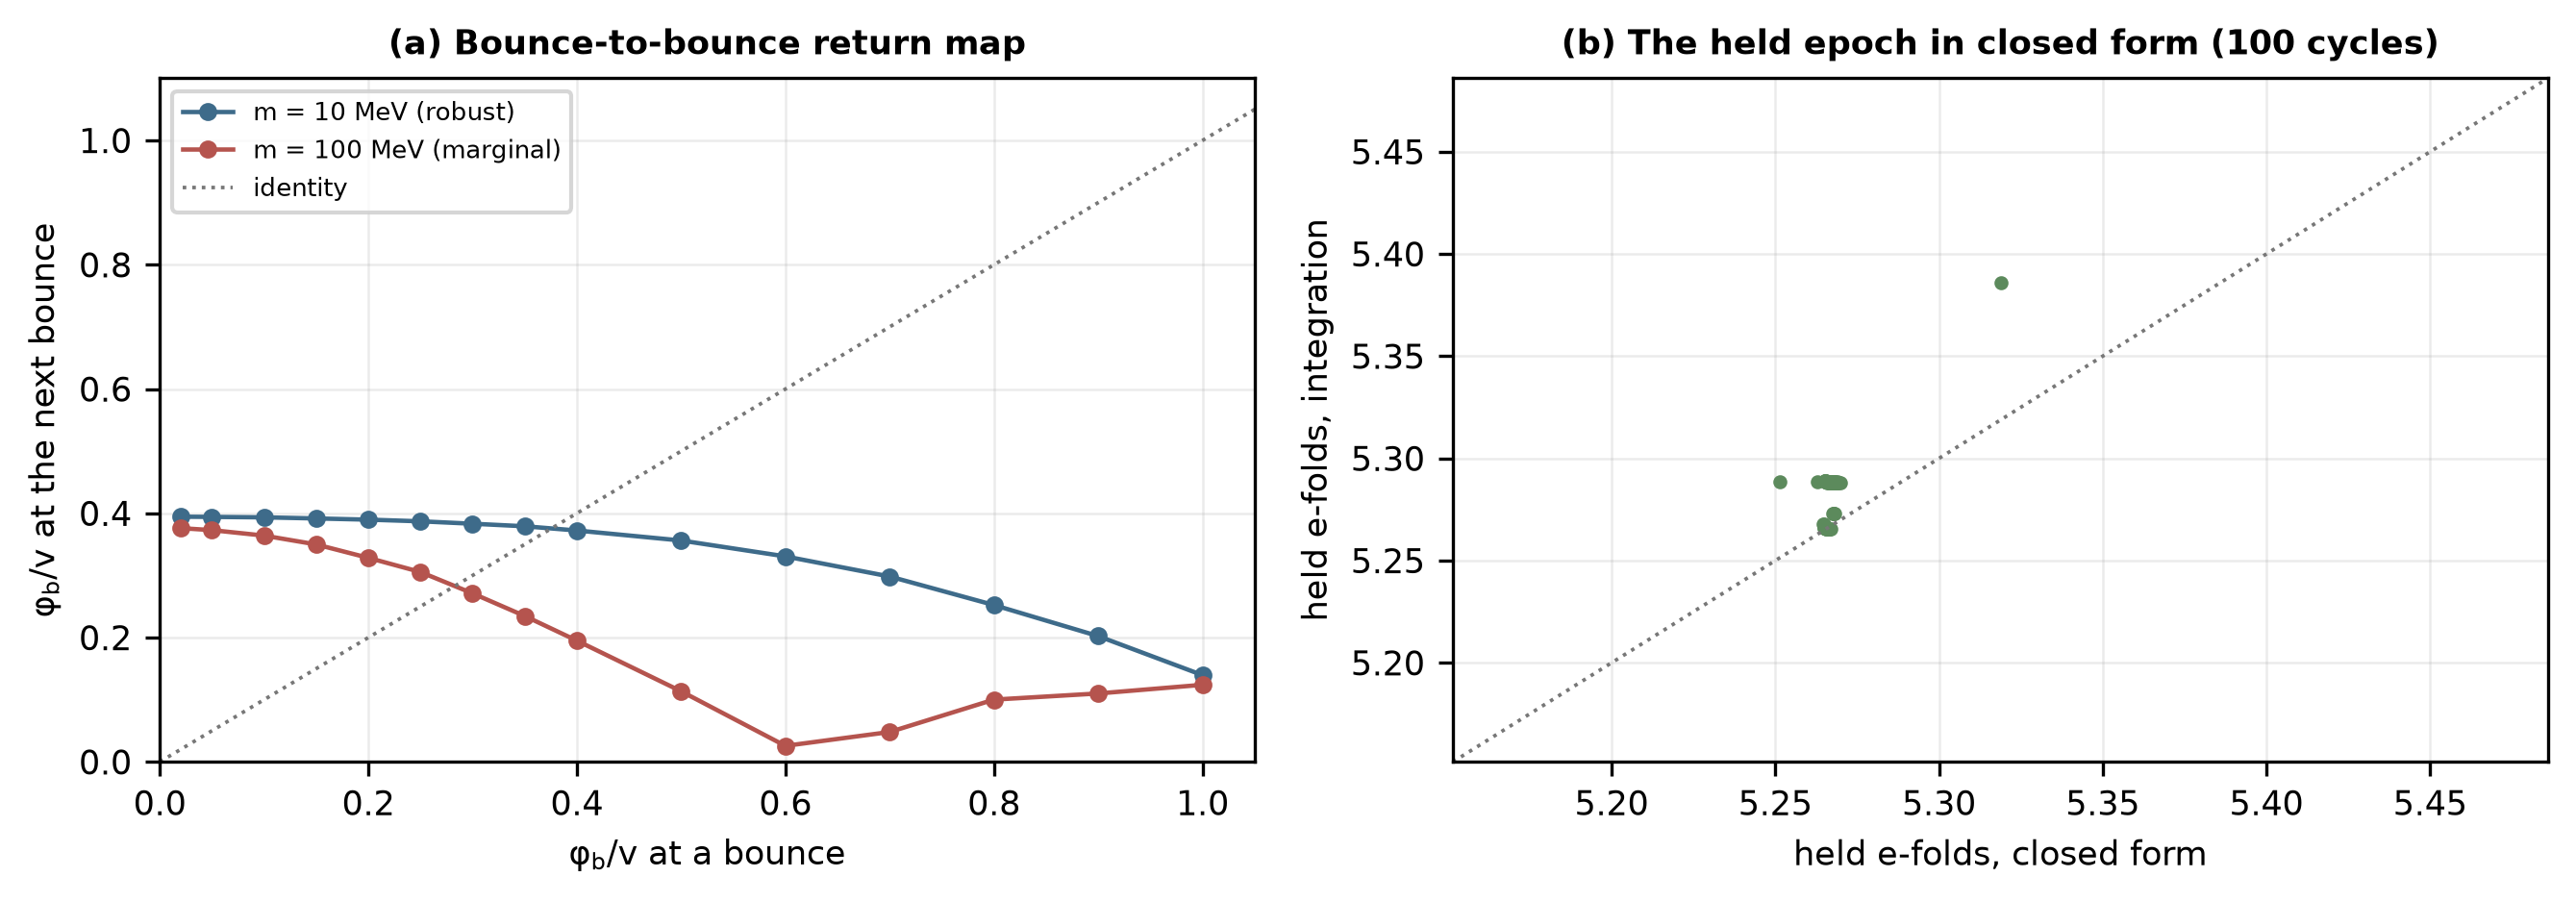
\includegraphics[width=1.00\textwidth]{../figures/fig18_cycle_map.png}\caption{(a) Bounce-to-bounce return map of the frozen field value for $m=10$ and 100 MeV (bounce at 172 MeV); dotted: the identity, whose intersection with each curve is the repeating cycle. (b) Held e-folds from the integration against the closed form, one point per cycle.}\end{figure}
\section{Numerical validation and parameter viability}
\subsection{Numerical method and the admissibility of its devices}
The cycle is integrated with the state $(\ln a, H, \varphi, \dot\varphi, T, N)$ and two auxiliary integrals (the radiation history and the pressure-volume work), in units of $H_0$ and $M_{\rm Pl}$. The integration proceeds in chunks of one doubling or halving of the scale factor with the clock restarted in each chunk, because near the bounce the time scale $\rho_c^{-1/2}$ is many orders of magnitude below the cycle time and an absolute clock cannot resolve it. Absolute tolerances are set relative to each variable, an eighth-order Runge--Kutta method is tried first with LSODA and Radau as fall-backs, the overdamped reduction is used where $\Upsilon>10^3\max(m_{\rm eff},H,\mu)$ (4331 chunks of the baseline run), and the constraint is projected away from the turning points (largest correction $1\times10^{-2}$). The Maxwell--Boltzmann integrals use the asymptotic series of the Bessel functions for $x>100$, where the library functions lose precision, and the heat capacity of the gas is computed analytically.

The results do not depend on how the numerical devices are set (numerics\_admissibility.py, three cycles per variant). A tighter tolerance ($10^{-10}$), a ten times stricter threshold for the overdamped reduction, and the constraint projection applied only at every fourth chunk change the held e-folds by at most 0.0033, the held-epoch abundance by at most 0.0048 and $\ln G_n$ by at most 0.00029 (relative), against a scatter between cycles of 0.0093, 0.073 and 0.00011 in the baseline itself; every variant is a working cycle. The projection cannot be removed altogether: without it the Friedmann-constraint residual grows to $3\times10^{37}$ through the stiff bounce and contraction phases and the integration stops before the first cycle closes. Projection keeps the integrator on the constraint surface, which the exact equations never leave, while its frequency does not matter (the residual rises from $6\times10^{-6}$ to $3\times10^{-4}$ when it is applied four times less often).

Two diagnostics must not be confused. The residual is the violation of the Friedmann constraint measured inside each chunk, normalized by the sum of the absolute values of the energy components; the projection correction is the relative change of $H$ applied at the start of a chunk. They differ by normalization, since $H$ is small wherever the components nearly cancel, and a small residual after projection does not by itself show that the unprojected trajectory is accurate. Table 3 lists both for every setting, together with the changes of the turnaround (its scale factor and the duration of the cycle) and of the cycle properties.

The decisive test is an independent formulation of the gravitational equations that needs no projection (independent\_solver.py). Away from the turning points $H$ is not integrated but computed from the constraint, $H=\pm[\rho(1-\rho/\rho_c)/3]^{1/2}$, so the constraint holds identically; close to a turnaround or bounce, where the square root carries no information about the change of sign, $H$ is evolved across a short bridge with the Raychaudhuri equation, entered when $H^2$ falls below a fixed fraction of the natural rate, and the constraint mismatch accumulated across each bridge is recorded. With the same matter equations, 3 of 3 settings of this solver complete three cycles; their bridges accumulate a mismatch of at most $1\times10^{-6}$, and they reproduce the projected integration to $4\times10^{-4}$ in the turnaround scale factor, $5\times10^{-4}$ in the duration of the cycle, $5\times10^{-3}$ in the held e-folds, $6\times10^{-3}$ in the held-epoch abundance and $3\times10^{-4}$ in $\ln G_n$. The projection is therefore not what makes the cycle repeat.

\begin{table}[htbp]\centering\footnotesize\setlength{\tabcolsep}{3pt}
\caption{Numerical diagnostics of the baseline (three cycles per setting; P: projected solver, C: constrained solver with the bridge parameter given). Residual: largest Friedmann-constraint violation inside a chunk; corrections: number and largest relative size of the projections of $H$ (projected solver) or the constraint mismatch at the end of the Raychaudhuri bridges (constrained solver); the last four columns give the largest relative change from the projected baseline in the turnaround scale factor, the duration of the cycle, the held e-folds and $\ln G_n$. The no-projection run stopped before the first cycle closed.}
\begin{tabular}{lllllllll}
\toprule
Setting & Outcome & Residual & Count & Max. corr. & $\ln a_{\max}$ & $t_{\rm cycle}$ & Held & $\ln G_n$ \\ \midrule
P: baseline & working & $6\times10^{-6}$ & 338 & $4\times10^{-3}$ & 0 & 0 & 0 & 0 \\
P: rtol $10^{-10}$ & working & $2\times10^{-7}$ & 331 & $2\times10^{-3}$ & $2\times10^{-4}$ & $3\times10^{-4}$ & $3\times10^{-3}$ & $3\times10^{-4}$ \\
P: overdamped $10^4$ & working & $6\times10^{-6}$ & 339 & $1\times10^{-3}$ & $4\times10^{-5}$ & $1\times10^{-4}$ & $3\times10^{-3}$ & $1\times10^{-4}$ \\
P: projection every 4th & working & $3\times10^{-4}$ & 83 & $1\times10^{-4}$ & $7\times10^{-5}$ & $1\times10^{-4}$ & $3\times10^{-3}$ & $1\times10^{-4}$ \\
P: no projection & failed & $3\times10^{37}$ & 0 & -- & -- & -- & -- & -- \\
C: bridge 0.05 & working & $1\times10^{-6}$ & 8 & $9\times10^{-7}$ & $4\times10^{-4}$ & $5\times10^{-4}$ & $3\times10^{-3}$ & $3\times10^{-4}$ \\
C: bridge 0.02 & working & $2\times10^{-6}$ & 8 & $1\times10^{-6}$ & $4\times10^{-4}$ & $5\times10^{-4}$ & $3\times10^{-3}$ & $3\times10^{-4}$ \\
C: bridge 0.05, rtol $10^{-10}$ & working & $5\times10^{-8}$ & 8 & $3\times10^{-8}$ & $4\times10^{-4}$ & $5\times10^{-4}$ & $5\times10^{-3}$ & $3\times10^{-4}$ \\
\bottomrule
\end{tabular}
\end{table}
\subsection{Where the cycles work, and how they fail}
Over a grid of dark-matter mass (1 MeV to 1 GeV) and bounce temperature (1.8 MeV to 1.8 GeV), with five cycles per run, the cycles work in 10 of 16 cells (Fig. 7b). Every failure in the grid is F1: the bounce is too cold to return the dark matter to equilibrium, the dark matter is annihilated in the contraction, and the next cycle has no matter to hold its vacuum. The dynamics are bistable: the field freezes at the bounce either at $\varphi_b\approx0.23$--$0.31v$, where the dark matter is light enough to rethermalize and the cycle reproduces itself, or near $v$, where it is $A(v)\approx85$ times heavier and is not regenerated. The condition that does not depend on the phase of the frozen field is a bounce that rethermalizes even the heaviest dark matter, $T_b\gtrsim mA(v)/5$. For $m=100$ MeV and $T_b=180$ MeV it is not met, and varying one parameter at a time about that point gives: $C_T=1000$: F1 dark matter not regenerated; $\mu/H_0=10$: F1 dark matter not regenerated; $a_c=3$: working; $q=3$: F1 dark matter not regenerated; $\mu/H_0=100$: F1 dark matter not regenerated; $\Omega_{\sigma,0}=10^{-10}$: F4 shear-dominated bounce; $q=0.3$: F1 dark matter not regenerated; $\Omega_{\sigma,0}=10^{-20}$: working; $a_c=1.5$: working; $C_T=0.001$: F1 dark matter not regenerated; $C_T=1e-06$: F6 wall-clock limit. For $m=10$ MeV at the same bounce it is met, and 6 of 8 variations work: $\mu/H_0=10$: working; $C_T=1000$: F2 vacuum not restored; $a_c=3$: working; $q=0.3$: working; $\mu/H_0=100$: working; $q=3$: working; $a_c=1.5$: working; $C_T=0.001$: F1 dark matter not regenerated. The classification looks for F1 (dark matter not regenerated), F2 (vacuum not restored), F3 (bounce dominated by the scalar's kinetic energy), F4 (bounce dominated by shear), F5 (no bounce) and F6 (numerical).

\subsection{Joint viability over parameter ranges}
How often are all the conditions met at once? Over stated ranges (viability\_mc.py; 200000 draws, log-uniform $a_c\in[0.5,10]$, $m\in[1,1000]$ MeV, $T_b\in[1\,{\rm MeV},10\,{\rm GeV}]$, uniform $q\in[-1,3]$) the vacuum is held today in 77\% of draws, recollapses in 75\%, has its bounce in the window between BBN and black-hole percolation in 66\%, and rethermalizes the dark matter, $T_b>mA(v)/5$ with the exact $A(v)$ of Section 2.1, in 34\%. All four hold together in 6.8\% of the draws, 11.7\% of those that are held today and recollapse; rethermalization is the binding condition. The window uses the baseline estimate of the black-hole bound; with the lower estimates of Section 4.5 the joint fraction falls to 2.5--5.7\%. Dissipation, a coherent seed and inherited rather than regenerated shear are required in addition and are not sampled. The fractions describe the sample space of the model, not a probability for our universe.

\subsection{Executable checks}
verify.py recomputes the checks of Table 4 from the stored results; the manuscript is built only if they pass. The repository also contains checks of an earlier tunneling analysis and of the companion interface paper, which are not used here.

\begin{table}[htbp]\centering\small
\caption{Executable checks of this paper (verify.py).}
\begin{tabular}{>{\raggedright\arraybackslash}p{0.086\dimexpr\textwidth-6\tabcolsep\relax}>{\raggedright\arraybackslash}p{0.819\dimexpr\textwidth-6\tabcolsep\relax}>{\raggedright\arraybackslash}p{0.095\dimexpr\textwidth-6\tabcolsep\relax}}
\toprule
No. & What is checked & Outcome \\ \midrule
V27 & matter-held vacuum: held today, release, recollapse; control fails & pass \\
V28 & prescribed-step hot cycles (earlier version) and their controls & pass \\
V29 & continuous cycles: 100 cycles with dark matter regenerated, matter era, held epoch; growth = entropy$^{1/3}$; cold bounce fails & pass \\
V30 & causal test: frozen matter never recollapses; diluting model recollapses for every $q>0$ & pass \\
V31 & shear scaling and ekpyrotic gain; bounce invariants and continuity; black-hole volume fraction & pass \\
V32 & attracting fixed point; closed-form held epoch; numerical devices; independent solver & pass \\
V33 & phase structure (spinodal release) and coherence of the release & pass \\
\bottomrule
\end{tabular}
\end{table}
\section{Observational constraints and limitations}
\subsection{Observational consequences}
\begin{itemize}\item Dark energy. While held, the vacuum has $1+w<8\times10^{-120}$; the model predicts no evolution of the dark energy before the release, the release near $a=a_c$ and a turnaround 94 Gyr from now for $a_c=2$, $\mu=30H_0$, $q=1$. A confirmed evolution of $w$ at the level suggested by recent baryon-acoustic-oscillation analyses [24] would exclude it.
\item Fifth forces and voids. The coupling vanishes at $\varphi=0$, so the homogeneous background and dense, collapsed structures carry no fifth force, and dark-matter perturbations do not source the field at linear order (Section 2.1). This is not a full equivalence with $\Lambda$CDM: the growth of structure at second order and in the time-dependent mass $m_{\rm eff}$ has not been computed. A void with density below $\rho_{\rm dm,0}/a_c^3$ and radius above the Compton length $\pi/\mu$ would release the vacuum locally today; void statistics bound the parameter space for large $\mu$ and small $a_c$.
\item Dark matter. The cycle requires a thermal relic rethermalized at the bounce: $m\lesssim5T_b/A(\varphi_b)$ and, with Section 4.5, $m$ below a few hundred MeV for $T_b\lesssim2.2$ GeV; a nonthermal dark matter (an axion produced by misalignment, for instance) or a heavier relic is incompatible with the cycle; thermal relics below a few MeV are separately constrained by BBN and the CMB [25].
\item Primordial perturbations. The scales observed today, $k=(1$--$1000)a_0H_0$, cross the Hubble radius of the preceding contraction at $T=25$--$32840$ (in units of 1.82 meV), where the contraction is radiation dominated ($w=0.333$). A contraction with constant $w$ gives $n_s-1=12w/(1+3w)$ [26, 27], i.e., $n_s=3.00$, with an amplitude set by $\rho_c/M_{\rm Pl}^4=3\times10^{-77}$, against $n_s=0.965$ and $2.1\times10^{-9}$ observed [28]. The background cycle does not produce the observed perturbations; a separate mechanism (for example a curvaton, or an entropic mechanism in an ekpyrotic phase) would be required, and none is part of this model.
\item Gravitational waves. Tensor modes from the contraction have the same tiny amplitude; the release is a homogeneous roll without bubble collisions; no primordial gravitational-wave signal is predicted.
\end{itemize}
\subsection{Consistency conditions and falsification tests}
The conditions the model must satisfy are of two kinds. Internal conditions, if violated, make the model ill defined; observational tests, if failed, disfavor it.

\begin{itemize}\item C1 (held vacuum). The vacuum is held today only if $a_c>1$, i.e., $\mu^2M^2<\rho_{\rm dm,0}$, and a release into a negative vacuum needs $A(v)-1=2(V_c-V_0(v))/\rho_{\rm crit}>2V_c/\rho_{\rm crit}$, a dark-matter mass that grows severalfold after the release (Section 2.1).
\item C2 (coherent release). The roll must be seeded coherently over the region, by a tilt $\epsilon\gtrsim4\times10^{-64}\,\mu^2v$ or an equivalent seed; otherwise domain walls form (Section 2.2).
\item C3 (dissipation). Repeated cycles are stable only if the dissipation per cycle exceeds the logarithm of the amplification of the scalar energy, $\Upsilon P\gtrsim\ln\mu$ (Section 4.2).
\item C4 (bounce window). The bounce must lie between BBN (5 MeV) and the percolation of the black holes of the previous cycle, estimated at 0.7--3.1 GeV within the population prescription and lower if accretion is much faster than geometric capture or the contraction strongly inhomogeneous (Section 4.5).
\item C5 (rethermalization). The bounce must return the dark matter to equilibrium, $T_b\gtrsim mA(v)/5$; otherwise the next cycle is empty (Sections 5.1, 6.2).
\item C6 (anisotropy). Shear regenerated in a cycle must stay below $2\times10^{-27}$ of the matter density at the turnaround, or an ekpyrotic phase must dilute it (Section 4.3).
\item O1 (dark energy). $w=-1$ exactly until the release; a confirmed evolution of $w$ excludes the model.
\item O2 (dark matter). A thermal relic below a few hundred MeV; a nonthermal or heavier dark matter excludes the cycle.
\item O3 (voids). The emptiest large voids must not release the vacuum today, which bounds large $\mu$ at small $a_c$.
\item O4 (perturbations). The observed spectrum must come from a mechanism outside the model; the model makes no prediction for $n_s$, $f_{\rm NL}$ or $r$.
\end{itemize}
\subsection{What is shown, and what is assumed}
\begin{table}[htbp]\centering\small
\caption{Status of the cyclic model.}
\begin{tabular}{>{\raggedright\arraybackslash}p{0.371\dimexpr\textwidth-6\tabcolsep\relax}>{\raggedright\arraybackslash}p{0.517\dimexpr\textwidth-6\tabcolsep\relax}>{\raggedright\arraybackslash}p{0.112\dimexpr\textwidth-6\tabcolsep\relax}}
\toprule
Element & Status & Where \\ \midrule
Vacuum held by matter, released by dilution & derived within the model; intervention test passed & 2, 3 \\
Turnaround & follows from $V_0(v)<0$; a negative vacuum alone also recollapses & 3.1, 3.3 \\
Coherent release & needs a seed or tilt $\epsilon\gtrsim4\times10^{-64}\,\mu^2v$ & 2.2 \\
Bounce & assumed (effective, far below the Planck density); a ghost-fluid bounce gives cycles but not self-similar ones & 4.1, 4.4, 4.6 \\
Reheating & continuous, no reset: dissipation $\Upsilon=C_TT^3$ (assumed form) and Boltzmann dark matter & 5.1 \\
Dark-matter abundance & output of freeze-out in every cycle; $\langle\sigma v\rangle$ fixed once by today & 5.1 \\
Vacuum restoration & output (frozen at the bounce, damped in the expansion) & 5.1, 5.2 \\
Entropy & grows each cycle; absorbed by Tolman growth $G_n=(S_{n+1}/S_n)^{1/3}$ & 5.1 \\
Anisotropy & inherited shear diluted by $G_n^6$; regenerated shear needs $s<10^{-27}$ or ekpyrosis & 4.3 \\
Black holes & estimated bound $T_b\lesssim$ 0.7--3.1 GeV (prescription dependent); relics diluted & 4.5 \\
$\Lambda$CDM past & homogeneous background only; perturbations and voids not tested & 2.1, 7.1 \\
Inhomogeneities, perturbations & not followed; the observed spectrum is not produced & 7.1 \\
Joint viability & 6.8\% of the sampled parameter space & 6.3 \\
\bottomrule
\end{tabular}
\end{table}
The limits are definite. The bounce is an effective prescription, and $\rho_c$ lies far below the Planck density in the simulations; the dissipation has an assumed form; the dynamics are homogeneous, so the growth of inhomogeneities in the contraction, which can dominate a contracting universe, is not followed (Bianchi I shear is the only anisotropy treated); the dark matter is a single species with Maxwell--Boltzmann statistics; and $a_c\sim1$ requires $\mu^2M^2\approx\rho_{\rm dm,0}$, a coincidence of the same kind as that of the cosmological constant. A first-order version of the trigger, in which the held vacuum becomes metastable and decays by bubble nucleation, is a distinct extension with its own questions and is not needed for the cycle reported here.

\section{Conclusions}
Within a stated model, the dilution of matter can end the cosmological expansion and, with an effective bounce, start a new hot phase. A scalar coupled to dark matter holds the observed dark energy with a homogeneous $\Lambda$CDM background and releases it by dilution into a negative vacuum; the expansion turns around, and an intervention that freezes the density seen by the field removes the turnaround. With an effective loop-quantum-cosmology bounce, dissipation and Boltzmann dark matter, 100 consecutive cycles were followed with no variable reset; in each, the dark matter is rethermalized and freezes out to the observed ratio, the vacuum is restored, held and released, and the entropy produced enlarges the next cycle by $(S_{n+1}/S_n)^{1/3}$. The repeating cycle is an attracting fixed point of the bounce-to-bounce map, and its dark-energy epoch has a closed form.

The conditions are explicit: a bounce at a fixed density, hot enough to rethermalize the dark matter and cold enough to keep the black holes of the previous cycle from percolating; dissipation; a thermal-relic dark matter; an anisotropy that is inherited rather than regenerated; and a coherent seed for the release. Over stated parameter ranges they hold together in 6.8\% of the sample space. With a colder bounce the cycle fails. The model does not produce the observed primordial perturbations, so these are conditional background solutions: they show what a cyclic hot big bang triggered by dilution requires, not that the universe has one.

Three extensions would test the framework further: a derivation of the bounce, or its replacement by a mechanism that fixes the bounce density from first principles; an inhomogeneous simulation of the contraction, in which the growth of structure rather than homogeneous shear decides whether the bounce is smooth; and a source of the primordial perturbations compatible with the cycle, for example an entropic mechanism in a contracting ekpyrotic phase. Each can falsify the model as it stands.

\section*{Declarations}
\noindent\textbf{Funding.} This research received no specific grant from funding agencies in the public, commercial, or not-for-profit sectors.

\noindent\textbf{Conflict of interest.} The author declares no competing interests.

\noindent\textbf{Data availability.} The data underlying every figure and table are in the repository listed below, as JSON and CSV files written by the scripts named in the text.

\noindent\textbf{Code availability.} All code (Python, NumPy, SciPy, Matplotlib [29, 30]) is at \url{https://github.com/sandlerleon/late-time-vacuum-decay} (MIT license) and archived at \url{https://doi.org/10.5281/zenodo.23841872}; this manuscript is archived at \url{https://doi.org/10.5281/zenodo.23841870}. Running the scripts in the order given in the README regenerates every number, table and figure.

\noindent\textbf{Related manuscript.} A companion manuscript on density-dependent vacuum bubble nucleation in the same class of matter-coupled models is in preparation for separate submission to Physics of the Dark Universe, archived at \url{https://doi.org/10.5281/zenodo.23841874}; it shares the class of models but none of the results reported here.

\noindent\textbf{Use of generative AI.} During the preparation of this work, the author used Claude (Anthropic) to assist with the design of the numerical analysis, code, literature checking and drafting. The author reviewed and edited all content and takes full responsibility for it.

\section*{References}
\noindent\hangindent=1.5em [1] R.C. Tolman, On the problem of the entropy of the universe as a whole. Phys. Rev. 37, 1639--1660 (1931). \url{https://doi.org/10.1103/PhysRev.37.1639}\par
\noindent\hangindent=1.5em [2] R. Penrose, Cycles of Time: An Extraordinary New View of the Universe. Bodley Head, London (2010).\par
\noindent\hangindent=1.5em [3] M. Gasperini, G. Veneziano, The pre-big bang scenario in string cosmology. Phys. Rep. 373, 1--212 (2003). \url{https://doi.org/10.1016/S0370-1573(02)00389-7}\par
\noindent\hangindent=1.5em [4] P.J. Steinhardt, N. Turok, A cyclic model of the universe. Science 296, 1436--1439 (2002). \url{https://doi.org/10.1126/science.1070462}\par
\noindent\hangindent=1.5em [5] A. Ijjas, P.J. Steinhardt, Bouncing cosmology made simple. Class. Quantum Grav. 35, 135004 (2018). \url{https://doi.org/10.1088/1361-6382/aac482}\par
\noindent\hangindent=1.5em [6] M. Novello, S.E. Perez Bergliaffa, Bouncing cosmologies. Phys. Rep. 463, 127--213 (2008). \url{https://doi.org/10.1016/j.physrep.2008.04.006}\par
\noindent\hangindent=1.5em [7] D. Battefeld, P. Peter, A critical review of classical bouncing cosmologies. Phys. Rep. 571, 1--66 (2015). \url{https://doi.org/10.1016/j.physrep.2014.12.004}\par
\noindent\hangindent=1.5em [8] J. Khoury, A. Weltman, Chameleon fields: awaiting surprises for tests of gravity in space. Phys. Rev. Lett. 93, 171104 (2004). \url{https://doi.org/10.1103/PhysRevLett.93.171104}\par
\noindent\hangindent=1.5em [9] K. Hinterbichler, J. Khoury, Screening long-range forces through local symmetry restoration. Phys. Rev. Lett. 104, 231301 (2010). \url{https://doi.org/10.1103/PhysRevLett.104.231301}\par
\noindent\hangindent=1.5em [10] K. Hinterbichler, J. Khoury, A. Levy, A. Matas, Symmetron cosmology. Phys. Rev. D 84, 103521 (2011). \url{https://doi.org/10.1103/PhysRevD.84.103521}\par
\noindent\hangindent=1.5em [11] L. Amendola, Coupled quintessence. Phys. Rev. D 62, 043511 (2000). \url{https://doi.org/10.1103/PhysRevD.62.043511}\par
\noindent\hangindent=1.5em [12] A. Ashtekar, T. Pawlowski, P. Singh, Quantum nature of the big bang. Phys. Rev. Lett. 96, 141301 (2006). \url{https://doi.org/10.1103/PhysRevLett.96.141301}\par
\noindent\hangindent=1.5em [13] A. Ashtekar, P. Singh, Loop quantum cosmology: a status report. Class. Quantum Grav. 28, 213001 (2011). \url{https://doi.org/10.1088/0264-9381/28/21/213001}\par
\noindent\hangindent=1.5em [14] P. Singh, Are loop quantum cosmos never singular? Class. Quantum Grav. 26, 125005 (2009). \url{https://doi.org/10.1088/0264-9381/26/12/125005}\par
\noindent\hangindent=1.5em [15] A. Berera, Warm inflation. Phys. Rev. Lett. 75, 3218--3221 (1995). \url{https://doi.org/10.1103/PhysRevLett.75.3218}\par
\noindent\hangindent=1.5em [16] E.W. Kolb, M.S. Turner, The Early Universe (Addison-Wesley, Redwood City, 1990)\par
\noindent\hangindent=1.5em [17] P. Gondolo, G. Gelmini, Cosmic abundances of stable particles: improved analysis. Nucl. Phys. B 360, 145--179 (1991). \url{https://doi.org/10.1016/0550-3213(91)90438-4}\par
\noindent\hangindent=1.5em [18] J. Pavlovic, N. Sossich, Geodesically complete cyclic cosmologies and entropy. Eur. Phys. J. C 84, 242 (2024). \url{https://doi.org/10.1140/epjc/s10052-024-12621-z}\par
\noindent\hangindent=1.5em [19] J. Khoury, B.A. Ovrut, P.J. Steinhardt, N. Turok, Ekpyrotic universe: colliding branes and the origin of the hot big bang. Phys. Rev. D 64, 123522 (2001). \url{https://doi.org/10.1103/PhysRevD.64.123522}\par
\noindent\hangindent=1.5em [20] V. Sahni, A. Toporensky, Cosmological hysteresis and the cyclic universe. Phys. Rev. D 85, 123542 (2012). \url{https://doi.org/10.1103/PhysRevD.85.123542}\par
\noindent\hangindent=1.5em [21] L. Sandler, Density-dependent vacuum bubble nucleation in matter-coupled dark-sector cosmology: wall dynamics, transmission and gravitational viability. Preprint, Zenodo (2026). \url{https://doi.org/10.5281/zenodo.23841874}\par
\noindent\hangindent=1.5em [22] J.K. Erickson, D.H. Wesley, P.J. Steinhardt, N. Turok, Kasner and mixmaster behavior in universes with equation of state w >= 1. Phys. Rev. D 69, 063514 (2004). \url{https://doi.org/10.1103/PhysRevD.69.063514}\par
\noindent\hangindent=1.5em [23] B.J. Carr, S.W. Hawking, Black holes in the early Universe. Mon. Not. R. Astron. Soc. 168, 399--415 (1974). \url{https://doi.org/10.1093/mnras/168.2.399}\par
\noindent\hangindent=1.5em [24] DESI Collaboration, M. Abdul Karim et al., DESI DR2 results. II. Measurements of baryon acoustic oscillations and cosmological constraints. Phys. Rev. D 112, 083515 (2025). \url{https://doi.org/10.1103/tr6y-kpc6}\par
\noindent\hangindent=1.5em [25] N. Sabti, J. Alvey, M. Escudero, M. Fairbairn, D. Blas, Refined bounds on MeV-scale thermal dark sectors from BBN and CMB. J. Cosmol. Astropart. Phys. 01, 004 (2020). \url{https://doi.org/10.1088/1475-7516/2020/01/004}\par
\noindent\hangindent=1.5em [26] D. Wands, Duality invariance of cosmological perturbation spectra. Phys. Rev. D 60, 023507 (1999). \url{https://doi.org/10.1103/PhysRevD.60.023507}\par
\noindent\hangindent=1.5em [27] F. Finelli, R. Brandenberger, Generation of a scale-invariant spectrum of adiabatic fluctuations in cosmological models with a contracting phase. Phys. Rev. D 65, 103522 (2002). \url{https://doi.org/10.1103/PhysRevD.65.103522}\par
\noindent\hangindent=1.5em [28] Planck Collaboration, Y. Akrami et al., Planck 2018 results. X. Constraints on inflation. Astron. Astrophys. 641, A10 (2020). \url{https://doi.org/10.1051/0004-6361/201833887}\par
\noindent\hangindent=1.5em [29] C.R. Harris et al., Array programming with NumPy. Nature 585, 357--362 (2020). \url{https://doi.org/10.1038/s41586-020-2649-2}\par
\noindent\hangindent=1.5em [30] P. Virtanen et al., SciPy 1.0: fundamental algorithms for scientific computing in Python. Nat. Methods 17, 261--272 (2020). \url{https://doi.org/10.1038/s41592-019-0686-2}\par
\end{document}